\documentclass[letterpaper,12pt]{article}
\usepackage{amsmath,amsfonts,amsthm,amssymb,graphicx,mathtools,tikz,hyperref}
\usepackage{esvect,esint, subcaption, mathrsfs,comment, quiver, faktor}
\usepackage[onehalfspacing]{setspace}
\usepackage[ddmmyyyy]{datetime}
\renewcommand{\dateseparator}{.}


% place figures and tables where it seems like they should be
\usepackage{float}
\floatplacement{figure}{H}
\floatplacement{table}{H}

% automatically center figures/tables
\makeatletter
\g@addto@macro\@floatboxreset{\centering}
\makeatother

\usepackage{tocvsec2}
\usepackage[bookmarksdepth=subsection]{hyperref}
\usepackage{bookmark}
\usepackage[margin=1in]{geometry}
\usepackage{authblk}
\usepackage{titling}
\setlength{\droptitle}{-1in}

\input{Library/Fonts/BlackboardBold.tex}
\input{Library/Fonts/MathCalligraphy.tex}
\input{Library/definitions.tex}
\theoremstyle{plain}
\newtheorem{theorem}{Teorema}
\newtheorem{axiom}{Axioma}
\newtheorem{lemma}[theorem]{Lema}
\newtheorem{proposition}[theorem]{Proposici\'on}
\newtheorem{postulate}{Postulado}
\newtheorem*{corollary}{Corolario}

\theoremstyle{definition}
\newtheorem*{definition}{Definici\'on}
\newtheorem{conjecture}{Conjetura}
\newtheorem{example}{Ejemplo}
\newtheorem*{homework}{Tarea}

\theoremstyle{remark}
\newtheorem*{claim}{Reclamo}
\newtheorem*{note}{Nota}


\pretitle{
    \begin{center}
        \fontsize{14pt}{1em}
        \bfseries\selectfont
            MATE6201-0U1 \\
            Prof. Luis A. Medina \\
            10.00 - 11.20 \\
            CNL-A-207 \\
            \vspace{14pt}
}

\posttitle{\end{center}}
\preauthor{\begin{center}\fontsize{12pt}{1em}\selectfont}
\postauthor{\end{center}}
\predate{\begin{center}\fontsize{12pt}{1em}\selectfont}
\postdate{\end{center}}

% section heading formatting
\renewcommand{\thesection}{\Roman{section}.}

\usepackage{sectsty}
\sectionfont{\centering\fontsize{12pt}{1em}\selectfont}

\title{Algebra Moderna}

%%%%%%%%%%%%%%%%%%%%%%%%%%%%%%%%%%%%%%%%%%%%%%%%%%%%%%%%%%%%%%%%%%%%%%%%%%%%%%%%
% Your names go here (one should be underlined)
%%%%%%%%%%%%%%%%%%%%%%%%%%%%%%%%%%%%%%%%%%%%%%%%%%%%%%%%%%%%%%%%%%%%%%%%%%%%%%%%
\author{Alec Zabel-Mena}
\affil{Universidad de Puerto Rico, Recinto de Rio Piedras}

\begin{document}
\maketitle
\section*{Lecture 1: Review}

We begin with a review of some prelimanary results of set theory and advanced
calculus.

\begin{definition}
    Let $A$ and $B$ be sets, and let $f:A \rightarrow B$ be a map of $A$ into
   $B$. We say that $f$ is  \textbf{1--1} if for every  $x,y \in X$,  $f(x)=f(y)$
   implies $x=y$. We say $f$ is \textbf{onto} if for every $y \in B$, there is
   an  $x \in A$ for which $y=f(x)$. We say that $f$ is a  \textbf{1--1
   correspondence} of $A$  \textbf{onto} $B$ if  $f$ is both 1--1 and onto and
   onto.
\end{definition}

\begin{theorem}[Beinstern's Theorem]\label{thm_1}
    Let $A$ and  $B$ be sets. If there is a 1--1 map of $A$ into  $B$, and a
    1--1 map of  $B$ into $A$, then there exists a 1--1 correspondence of
    $A$ onto  $B$.
\end{theorem}

\begin{axiom}[The Axiom of Choice]\label{axm_1}
    Suppose that $\{A_\alpha\}_{\alpha \in \Lambda}$ is a collection of nonmepty
    sets indexed by the set $\Lambda$. Then there exists a map $f:\Lambda
    \rightarrow \bigcup{A_\alpha}$ called a \textbf{choice function}, defined by
    the rule $f(\alpha) \in A_\alpha$ for all $\alpha \in \Lambda$.
\end{axiom}
\begin{remark}
    What this axiom says is that given any (not necesarrily countable)
    collection of sets, one can ``choose '' an element from each set.
\end{remark}

\begin{definition}
    We define an \textbf{order} on a set $A$ to be a relation  $<$ satisfying
    the following properties for all $a,b,c \in A$:.
    \begin{enumerate}
        \item[(1)] $a<a$  (Reflexive).

        \item[(2)] If $a<b$ and  $b<a$, then  $a=b$  (Antisymmetry).

        \item[(3)] If $a<b$ and  $b<c$, then  $a<c$  (Transitivity).
    \end{enumerate}
     We say that elements $a,b \in A$ are \textbf{comparable} under $<$ if
     either $a<b$ or $b<a$. If every element of $A$ is comparable, then  $<$ is
     called a  \textbf{total order}.
\end{definition}

\begin{definition}
    Let $A$ be a set with order  $<$. We call an element  $x \in A$ a
    \textbf{maximum} of $A$ if  $x<a$ implies  $x=a$ for all $a \in A$. If $B
    \subseteq A$, then we call an element $a \in A$ an \textbf{upper bound} of
    $B$ if  $b<a$ for all  $B$ in  $B$; and we say  $B$ is  \textbf{bounded
    above}. If $b<a'$ implies that  $a<a'$ for any  $a' \in A$, then we call
    $a$ a  \textbf{least upper bound} of $B$ and write  $\sup{B}=a$.
\end{definition}

\begin{definition}
    Let $A$ be a set with order  $<$. We call an element  $x \in A$ a
    \textbf{minimum} of $A$ if  $a<x$ implies  $x=a$ for all $a \in A$. If $B
    \subseteq A$, then we call an element $a \in A$ an \textbf{lower bound} of
    $B$ if  $a<b$ for all  $B$ in  $B$; and we say  $B$ is  \textbf{bounded
    below}. If $a'<b$ implies that  $a'<a$ for any  $a' \in A$, then we call
    $a$ a  \textbf{greatest lower bound} of $B$ and write  $\inf{B}=a$.
\end{definition}

\begin{theorem}[Zorn's Lemma]\label{thm_2}
    Let $A$ be a set with order  $<$. If every totally ordered subset of  $A$
    under  $<$ has an upperbound, then  $A$ has a maximum element.
\end{theorem}
\begin{remark}
    It can be shown that Zorn's lemma and the axiom of choice are equivalent
    statements. That is you can prove Zorn's lemma from the axiom of choice, and
    you can prove the axiom of choice from Zorn's lemma.
\end{remark}

\begin{theorem}\label{thm_3}
    For any sets $A$ and  $B$, there is either a 1--1 map of  $A$ into  $B$, or
    a 1--1 map of  $B$ into  $A$.
\end{theorem}
\begin{proof}
    Consider the collection of all triples $C=\{(X,Y,f) : f:X \rightarrow Y
    \text{ is 1--1 and onto, where }\\ X \subseteq A, Y \subseteq B\}$, and
    define an order $<$ on  $C$ by: $(X,Y,f)<(X',Y',g)$ if, and only if $X
    \subseteq X'$,  $Y \subseteq Y'$, and  $g|_X=f$. Now suppose that the
    collection  $\{(X_\alpha, Y_\alpha,f_\alpha)\}$ is a totally ordered subset
    of $C$. Then define
    \begin{align*}
        \tilde{X}   &=      \bigcup_{\alpha}{X_\alpha} \\
        \tilde{Y}   &=      \bigcup_{\alpha}{Y_\alpha} \\
    \end{align*}
    and since for all $x \in \tilde{X}$, there is an $\alpha$  for which $x \in
    X_\alpha$, define the map $\tilde{f}:\tilde{X} \rightarrow \tilde{Y}$ by the
    rule $\tilde{f}(x)=f_\alpha(x) \in Y_\alpha$. This map is well defined by
    the total order on $\{(X_\alpha,Y_\alpha,f_\alpha)\}$.

    Now, notice that $\tilde{f}$ is an upperbound of the collection
    $\{(X_\alpha,Y_\alpha_f_\alpha)\}$, therefore, by Zorn's lemma there is a
    maximum element $(X,Y,f)$ of $C$. By definition we get that $f$ is a 1--1
    correspondence of $X$ onto $Y$, and by maximality, we get that either $X=A$
    or $Y=B$. Suppose on the contary that this is not true. Then there is an  $a
    \in \com{A}{X}$ and a $b \n \com{B}{Y}$. Letting $X'=X \cup a$ and  $Y'=Y
    \cup b$, and  $f':X' \rightarrow Y'$ defined by $f'|_X=f$ and  $f'(a)=b$.
    Then $(X,Y,f)<(X',Y',f')$, which contradicts the maximality of $(X,A,f)$.

    Therefore, we must have that either $X=A$ or  $Y=B$. Now, if  $X=A$, then
    $f:A \rightarrow Y$ is 1--1 and onto, taking the extension of $Y$ to  $B$,
    $f_B:A \rightarrow B$, we see it must be 1--1 as well. By the same reasoning
    we can assure there is a 1--1 map $f_A:B \rightarrow A$ of $B$ into  $A$.
\end{proof}

\section*{Lectura 2: Demostraci\'on General del Teorema de Puntos Fijos de
Brouwer}

\begin{definition}
    Sea $X$ un subsepacio de un espacio topologico  $Y$. Decimos que  $X$ es un
     \textbf{retracto} de $Y$ s\'i existe una mapa continua $r:Y \rightarrow X$
     donde $r(x)=x$ para todo $x \in X$. Llamamos a $r$ una
     \textbf{retracci\'on} de $Y$ sobre  $X$.
\end{definition}

Es decir que el retracci\'on de $Y$ sobre $X$  lleva sus puntos fijos en todo el
$X$. Podemos ver que  $r$ es una mapa sobre, ya que $r(X)=X$ por definici\'on.

\begin{figure}[h]
    \centering
    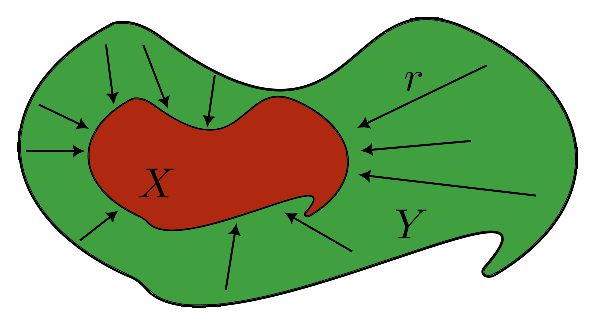
\includegraphics[scale=1.0]{Figures/retract_diagram.eps}
    \caption{Un retracci\'on $r:Y \rightarrow X$ de un espacio $Y$ hac\'ia un
    espacio  $X$.}
    \label{fig_3}
\end{figure}

Ahora recuerda que las mapas de inclusi\'on y identidad para espacios
topol\'ogicos son las mapas $i:X \rightarrow Y$ (donde $X$ es subespacio de
$Y$), y $1_X:X \rightarrow X$ dado por $i:x \rightarrow x$ y $1_X:x \rightarrow
x$ para todo $x \in X$. La definici\'on del retracto entonces se puede ver en la
siguiente diagrama, llamado una diagrama ``commutativa'':
\[\begin{tikzcd}
	&& Y \\
	\\
	\\
	X &&&& X
	\arrow["i", from=4-1, to=1-3]
	\arrow["{1_X}"', from=4-1, to=4-5]
	\arrow["r", dashed, from=1-3, to=4-5]
\end{tikzcd}\]
Entonces, seg\'un esta diagrama, $r \circ i=1_X$.

Dado una diagrama commutativa en el ``universo`` de espacios topologicos,
entonces queremos que las mapas sean mapas continuas. En este ejemplo, existe
una ``meta funci\'on`` llamado un ``functor'' $\Fc$ que lleva las espacios
topologicos hacia grupos Abelianos, tal que las diagramas commutativas son
preservada; es decir,  $\Fc$ lleva mapas continuas hacia homomorfismos.

 \begin{figure}[h]
    \centering
\[\begin{tikzcd}
	A &&&& B \\
	\\
	\\
	\\
	C
	\arrow["f", from=5-1, to=1-1]
	\arrow["g", from=1-1, to=1-5]
	\arrow["h"', from=5-1, to=1-5]
\end{tikzcd}\]
    \caption{Una diagrama commutativa, donde $A$, $B$,  $C$ son conjuntos
    cualquieras, y $f$,  $g$, y  $h$ son funciones cualquieras doned  $f \circ
g=h$.}
    \label{fig_4}
\end{figure}

\begin{lemma}\label{lemma_2.2}
    S\'i $n \geq 0$, entonces  $S^n$ no es un retracto de  $D^{n+1}$.
\end{lemma}
\begin{proof}
    Para $n=0$, es facil ver. Si  $r:D^1 \rightarrow S^0$ es un retracto,
    entonces la siguente diagrama
    \[\begin{tikzcd}
	&& {D^1} \\
	\\
	\\
	{S^0} &&&& {S^0}
	\arrow["i", from=4-1, to=1-3]
	\arrow["{1_{S^0}}"', from=4-1, to=4-5]
	\arrow["r", dashed, from=1-3, to=4-5]
\end{tikzcd}\]
nos da $r \circ i=1_{S^0}$ lo cual es imposible, ya que $S^0$ no es con\'exo, y
la imagen de  $D^1$ como subsepacio de  $S^0$ si lo es; es decir que
$r(D^1)=\{1\}$, \'o $r(D^1)=\{-1\}$. Entonces $r$ no puede ser  1--1 y sobre lo
cual contradice que  $r \circ i=1_{S^0}$ sea 1--1 y sobre.

Ahora, toma $n>0$, entonces suponga que exista una retracci\'on  $r:D^{n+1}
\rightarrow S^n$, con su diagrama de espacios topologicos y mapas continuas.
\[\begin{tikzcd}
	&& {D^{n+}} &&&&&& {H_n(D^{n+1})} \\
	\\
	\\
	{S^n} &&&& {S^n} && {H_n(S^n)} &&&& {H_n(S^n)}
	\arrow["i", from=4-1, to=1-3]
	\arrow["r", from=1-3, to=4-5]
	\arrow["{1_{S^n}}"', from=4-1, to=4-5]
	\arrow["{H_n(i)}", from=4-7, to=1-9]
	\arrow["{H_n(r)}", from=1-9, to=4-11]
	\arrow["{H_n(1_{S^n})}"', from=4-7, to=4-11]
\end{tikzcd}\]
Entonces $r \circ i=1_{s^n}$. Aplicando un functor particular llamado $H_n$,
obtemeos una diagrama commutativa de grupos Abelianos y homomorfismos. Las dos
diagramas se pueden ver arriba. Entonces tenemos que $H_n(S^n)=\Z$, y
$H_n(D^{n+1})=\vbrack{0}$. Ahora tenemos que $H_n(r) \circ
H_n(i)=H_n(1_{S^n})=1_\Z$. Esto es imposible ya que $1_\Z$ no se facotriza sobre
$\vbrack{0}$; i.e. $H_n(r) \circ H_n(i)=0 \ne 1_\Z$. Por lo tanto $S^n$ no
puede ser un retracto de  $D^{n+1}$.
\[\begin{tikzcd}
	&& \langle0\rangle \\
	\\
	\\
	\Z &&&& \Z
	\arrow["{H_n(i)}", from=4-1, to=1-3]
	\arrow["{H_n(r)}", from=1-3, to=4-5]
	\arrow["{1_\Z}"', from=4-1, to=4-5]
\end{tikzcd}\]
\end{proof}

Ahora reiteremos la teorema de Brouwer para la demostraci\'on para $n$ general.

\begin{theorem}[Teorema de Puntos Fijos de Brouwer]
    S\'i $f:D^n \rightarrow D^n$ es una funci\'on continua, entonces existe un
    punto fijo en $D^n$ para toda $n \geq 1$.
\end{theorem}
\begin{proof}
    Para $n>1$, suponga que no hay puntos fijos. Entonces sea $f:D^n \rightarrow
    D^n$ y que $f(x) \neq x$ para todo $x \in D^n$. Defina entonces, la mapa
    $g:D^n \rightarrow S^{n-1}$ dado por la figura \ref{fig_5}.
    \begin{figure}[h]
        \centering
        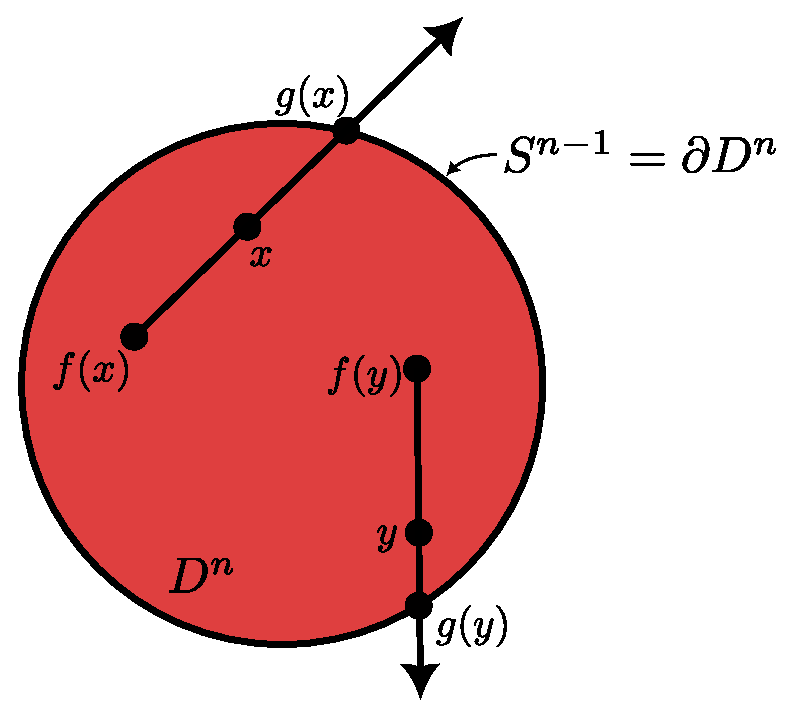
\includegraphics[scale=0.5]{Figures/brouwer_thm_2.eps}
        \caption{}
        \label{fig_5}
    \end{figure}
    Note que $g$ es continua, y que  $g(x)=x$ para todo $x \in S^{n-1}$. Puse,
    vemos que $g$ es una retracci\'on, lo cual es imposible por el lema
    \ref{lemma_2.2} Por lo tanto, no existen puntos fijos.
\end{proof}

\section*{Lectura 3: Categor\'ias y Funtores.}

\begin{definition}
    Definimos una \textbf{clase} de ser una colecci\'on de objetos tal que s\'i
    $T$ y  $A$ son clases, entonces  $A \notin T$.
\end{definition}

\begin{definition}
    Una \textbf{categor\'ia} $\Cc$ es un clase de objetos denotados por
    $\obj{\Cc}$ junto a una colecci\'on de conjuntos $\Hom{(X,Y)}$,  para
    cualquieras $X,Y \in \obj{\Cc}$, de \textbf{morfismos} de $X$ hac\'ia $Y$,
    cuyas elementos estan denotados $f:X \rightarrow Y$ \'o $X \xrightarrow{f}
    Y$, y una operac\i\'on binaria $\circ:\Hom{(X,Y)} \times \Hom{(Y,Z)}
    \rightarrow \Hom{(X,Z)}$ llamado \textbf{composici\'on} tal que si $f:X
    \rightarrow Y$ y $g:Y \rightarrow Z$ son morfismos, entonces $g \circ f:X
    \rightarrow Z$ es un morfismo y:
    \begin{enumerate}
        \item[(1)] $\Hom{(X,Y)}$ y $\Hom{(A,B)}$ son disjuntas.

        \item[(2)] La composici\'on $\circ$ es associativa s\'i esta definido.
            Es decir, sy  $g \circ (f \circ h)$ \'o $(g \circ g) \circ h$
            existen en $\Hom{(X,Y)}$, entonces $g \circ (f \circ h)=(g \circ f)
            \circ g$.

        \item[(3)] $\Hom{(X,X)}$ no es vac\'io y existe al menos un morfismo
            $1_X:X \rightarrow X$, llamado la \textbf{identidad} de $X$, tal que
            $1_X \circ f=f$ y  $g \circ 1_X=g$ para morfismos  $f:X \rightarrow
            Y$ y $g:Z \rightarrow X$, para cualquieras objetos $X,Y,Z \in
            \obj{\Cc}$
    \end{enumerate}
\end{definition}

\begin{definition}
    Sea $\Cc$ una categor\'ia. Se llama el conjunto $\Mc_\Cc$  \textbf{los
    morfismos de la categor\'ia} donde $\Mc_\Cc$ es la union de todos los
    conjuntos $\Hom{(X,Y)}$ para todos $X,Y \in \obj{\Cc}$.
\end{definition}

\begin{figure}[h]
    \centering
    \[\begin{tikzcd}
	X &&& Y &&& Z
	\arrow["f", from=1-1, to=1-4]
	\arrow["g", from=1-4, to=1-7]
	\arrow["{g \circ f}"', curve={height=30pt}, from=1-1, to=1-7]
\end{tikzcd}\]
    \caption{Un ejemplo de composici\'on de morfismos de una categor\'ia}
    \label{fig_6}
\end{figure}

\begin{figure}[h]
    \centering
    \[\begin{tikzcd}
	X & X &&& Y & Y
	\arrow[curve={height=12pt}, from=1-2, to=1-5]
	\arrow[curve={height=-12pt}, from=1-2, to=1-5]
	\arrow[from=1-2, to=1-5]
	\arrow["{1_X}", from=1-2, to=1-1]
	\arrow["{1_Y}", from=1-5, to=1-6]
	\arrow[curve={height=24pt}, from=1-5, to=1-2]
	\arrow[curve={height=-24pt}, from=1-5, to=1-2]
\end{tikzcd}\]
    \caption{Morfismos entre dos objetos $X$ y  $Y$ de una categor\'ia
    incluyendo las identidades de $X$ y $Y$}
    \label{fig_7}
\end{figure}

\begin{example}\label{}
    \begin{enumerate}
        \item[(1)] Considere la categor\'ia $\Cc=\Conj$, donde  $\boj{\Cc}$ es
            la clase de todo los conjuntos. Los morfismos de $\Cc$ son
            funci\'ones  $f:X \xrightarrow{} Y$ de un conjunto $X$ hac\'ia un
            conjunto  $Y$.

        \item[(2)] Sea $\Cc=\Top$ la categor\'ia de espacios topol\'ogicos,
            donde  $\obj{\Cc}$ es la colecci\'on de todas las espacios
            topol\'ogicos. Los morfismos de $\Top$ son funci\'ones continuas
            entre espacios topologicos. Es decir, $\Hom{(X,Y)}=\{f : f:X
            \xrightarrow{} Y \text{ es continua}\}$. La composici\'on de
            morfismos es la composicion de funciones usual.

        \item[(3)] Sea $\Cc=\Grp$ la categor\'ia de grupos, cuyas objetos son
            todo los grupos. Entonces los morfismos de  $\Grp$ estan definido
            por los conjuntos  $\Hom{(G,H)}=\{\phi : \phi:G \xrightarrow{} H
            \text{ es un homomrfismo}\}$. La composici\'on de morfismos es la
            composicion de funciones usual.
    \end{enumerate}
\end{example}

\begin{definition}
    Sean $\Cc$ y  $\Ac$ categor\'ias con  $\obj{\Cc} \subseteq \obj{\Ac}$.
    Decimos que $\Cc$ es una \textbf{subcategor\'ia} de $\Ac$ s\'i
    $\Hom_\Cc{(X,Y)} \subseteq \Hom_\Ac{(X,Y)}$ para todo $X,Y \in \obj{\Cc}$ ty
    la composici\'on de $\Cc$ es la misma de  $\Ac$.
\end{definition}

\begin{example}\label{}
    \begin{enumerate}
        \item[(1)] Tenemos que $\Top$ y  $\Grp$ son subcategor\'ias de
            $\Conj$.
        \item[(2)] La categor\'ia $\Top^2$ de pares topologicos tiene como objetos
            son todas pares  $(X,A)$, donde $X$ es un espacio topol\'ogico y $A
            \subseteq X$ es subsepacio de $X$. Los morfismos de $\Top^2$, para
            pare topologicos  $(X,Y)$ y $(Y,B)$, son las funciones continuas
            $f:X \xrightarrow{} Y$ donde $f(A) \subseteq B$ es subespacio de $B$.

        \item[(3)] La categor\'ia $\Top^*$ de pares topologicos  $(X,a)$, donde
            $a$ es un punto en  $X$ es una subcategor\'ia de  $\Top^2$.
    \end{enumerate}
\end{example}

\begin{definition}
    Sea $\Cc$ una categor\'ia. Una \textbf{diagrama} de objetos y morfismos en
    $\Cc$ es un grafo dirigido cuya cunjunto de vertices es subconjunto de
    $\obj{\Cc}$ y cuyas aristas son morfismos entre esos vertices. Decimos que
    una diagrama es \textbf{commutativo} si para cualquieras vertices $A,B,C,D$
    en la diagrama, y cualquier morfismos  $f:A \xrightarrow{} B$, $i:C
    \xrightarrow{} D$, $h:A \xrightarrow{} C$, y $g:B \xrightarrow{} D$, tenemos
    que $g \circ f=i \circ h$.
\end{definition}

\begin{example}\label{}
    Las figuras \ref{fig_6} y \ref{fig_7} son ejemplos de diagramas de objetos y
    morfismos en una categori\'ia.
\end{example}

\begin{figure}[h]
    \centering
    \[\begin{tikzcd}
	A &&&&& B \\
	\\
	\\
	C &&&&& D
	\arrow["f", from=1-1, to=1-6]
	\arrow["i", from=4-1, to=4-6]
	\arrow["g", from=1-6, to=4-6]
	\arrow["h"', from=1-1, to=4-1]
	\arrow["{g \circ f=i \circ h}", dashed, from=1-1, to=4-6]
\end{tikzcd}\]
    \caption{Un diagrama commutativa entre objetos y morfismos de una
    categor\'ia.}
    \label{fig_8}
\end{figure}

\section*{Lectura 3: Categor\'ias y Funtores.}

\section*{Lectura 5: Teoremas de Isomorfismo.}

\[\begin{tikzcd}
	& {\faktor{\Z}{24\Z}} &&&&&& \Z \\
	{\langle 2 \rangle} && {\lang 3 \rang} && 2\Z & 3\Z & 5\Z & 7\Z & \dots \\
	{\lang 4 \rang} && {\lang 6 \rangle} && 4\Z & 6\Z & 9\Z & 10\Z & \dots \\
	{\langle 8 \rangle} && \langle12\rangle && 8\Z & 12\Z & 18\Z & 20\Z & \dots \\
	& {\langle 0 \rangle} &&& \vdots & 24\Z & \vdots & \vdots & \dots
	\arrow[no head, from=1-2, to=2-1]
	\arrow[no head, from=2-1, to=3-1]
	\arrow[no head, from=3-1, to=4-1]
	\arrow[no head, from=4-1, to=5-2]
	\arrow[no head, from=5-2, to=4-3]
	\arrow[no head, from=4-3, to=3-1]
	\arrow[no head, from=4-3, to=3-3]
	\arrow[no head, from=3-3, to=2-3]
	\arrow[no head, from=2-3, to=1-2]
	\arrow[no head, from=2-1, to=3-3]
	\arrow[no head, from=1-8, to=2-5]
	\arrow[no head, from=1-8, to=2-6]
	\arrow[no head, from=1-8, to=2-7]
	\arrow[no head, from=1-8, to=2-8]
	\arrow[no head, from=1-8, to=2-9]
	\arrow[no head, from=2-5, to=3-5]
	\arrow[no head, from=2-5, to=3-6]
	\arrow[no head, from=2-5, to=3-8]
	\arrow[no head, from=2-5, to=3-9]
	\arrow[no head, from=2-6, to=3-6]
	\arrow[no head, from=2-6, to=3-7]
	\arrow[no head, from=2-6, to=3-9]
	\arrow[no head, from=3-5, to=4-5]
	\arrow[no head, from=3-5, to=4-6]
	\arrow[no head, from=3-5, to=4-8]
	\arrow[no head, from=3-5, to=4-9]
	\arrow[no head, from=4-5, to=5-5]
	\arrow[no head, from=4-7, to=5-8]
	\arrow[no head, from=4-7, to=5-9]
	\arrow[no head, from=4-6, to=5-6]
	\arrow[no head, from=4-5, to=5-6]
	\arrow[no head, from=4-6, to=5-8]
	\arrow[no head, from=4-7, to=5-7]
	\arrow[no head, from=3-6, to=4-6]
	\arrow[no head, from=3-6, to=4-8]
	\arrow[no head, from=3-6, to=4-9]
	\arrow[no head, from=4-6, to=5-9]
\end{tikzcd}\]

\[\begin{tikzcd}
	& \Z \\
	2\Z && 3\Z \\
	4\Z && 6\Z \\
	8\Z && 12\Z \\
	& 24\Z
	\arrow[no head, from=1-2, to=2-1]
	\arrow[no head, from=2-1, to=3-3]
	\arrow[no head, from=3-3, to=4-3]
	\arrow[no head, from=4-3, to=3-1]
	\arrow[no head, from=3-1, to=4-1]
	\arrow[no head, from=4-1, to=5-2]
	\arrow[no head, from=5-2, to=4-3]
	\arrow[no head, from=3-3, to=2-3]
	\arrow[no head, from=2-3, to=1-2]
	\arrow[no head, from=2-1, to=3-1]
\end{tikzcd}\]

\section*{Lectura 6: La Teoreman Fundamental del Algebra.}

\begin{theorem}[La Teorema Fundamental del Algebra]\label{thm_6.11}
    Todo polinomio con coeficientes complejas tiene al menos una ra\'iz
    complejo.
\end{theorem}
\begin{proof}
    Sea $\Sigma_\rho \subseteq \C$ el circulo de radio  $\rho$ en  $\C$.
    Considere la mapa  $f:\C \xrightarrow{} \C$ dado por $f(z)=z^n$, y denota
    $f^n_\rho=f|_{\Sigma_\rho}$. Nota que los $f^n_\rho$ son homotopicamentes
    nulas.

    Ahora, considere el polinomio  $g(z)=z^n+a_{n-1}z^{n-1}+\dots+a_1z+a_0$
    donde $a_i \in \C$ para todo  $0 \leq i \leq n$ y  $\deg{g}=n \geq 1$.
    Escoga $\rho>\max{\{1,\sum{|a_i|}\}}$, y defina la mapa $F:\Sigma_\rho
    \times I \xrightarrow{} \C$ dado por
    \begin{equation*}
        F(z,t)=z^n+\sum_{i=0}^{n-1}{(1-t)a_iz^i}
    \end{equation*}
    Por la contunuidad de polinomios en $\C$, tenemos que  $F$ es continua. Mas
    a\'un tenemos que  $F(z,0)=z^n+a_{n-1}z^{n-1}+\dots+a_1z_1+a_0=g(z)$ y
    $F(z,1)=z^n=f^n_\rho$. As\'i que $f^n_\rho \simeq g$ son homotopicos atraves
    de la homotopia $F$.

    Afirmamos que $F(z,t) \neq 0$. Por lo contrario, asuma que existe un $(z,t)
    \in \Sigma_\rho \times I$ tal que $F(z,t)=0$. Entonces tenemos que
    \begin{equation*}
        z^n=-\sum_{i=0}^{n-1}{(1-t)a_iz^i}
    \end{equation*}
    Por la desigualdad de triangulo, tenemos
    \begin{equation*}
        |z^n|=\rho^n \leq \sum{(1-t)|a_i|\rho^i} \leq \rho^{n-1}\sum{(1-t)|a_i|}
    \end{equation*}
    como $\rho>1$ y  $t \in I$ implica que  $\sum{(1-t)|a_i|} \leq \sum{|a_|}$,
    tenemos que
    \begin{equation*}
        \rho \leq \sum_{i=0}^{n-1}{(1-t)|a_i|}
    \end{equation*}
    lo cual contradice neustor escojido de $\rho$. Asi que  $F(z,t) \neq 0$ para
    todos $(z,t) \in \Sigma_\rho \times I$.

    \begin{figure}[h]
        \centering
        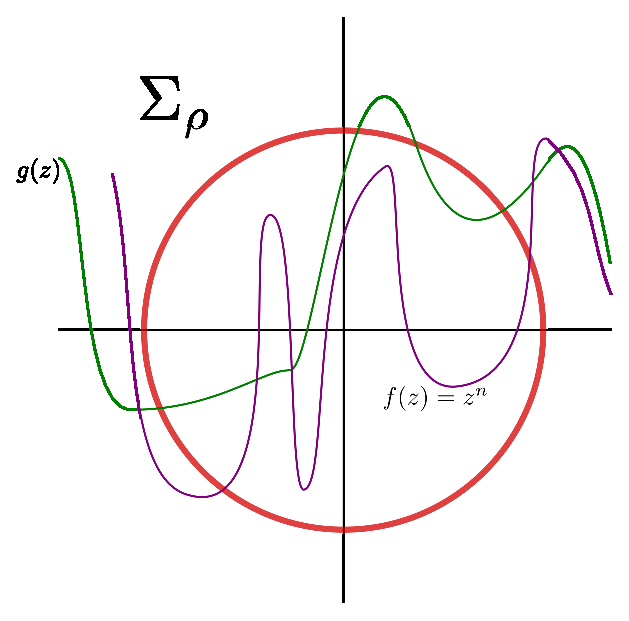
\includegraphics[scale=0.5]{Figures/fund_thm_algebra.eps}
        \caption{La teorema Fundamental del Algebra. Nota que $f^n_\rho$ consiste de
        cuyas puntos de $f(z)=z^n$ cuyas puntos intersecan con $\Sigma_\rho$.}
        \label{fig_16}
    \end{figure}

    Finalmente, tenemos que $F:\Sigma_\rho \times I \xrightarrow{}
    \com{\C}{\{0\}}$. Entonces suponga que $g(z)$ no tiene raices complejas.
    Defina $G:\Sigma_\rho \times I \xrightarrow{} \com{\C}{\{0\}}$ dado por
    $G(z,t)=g((1-t)z)$. Tenemos que $(1-t)z$ es una mapa continua, y que $g$ es
    continua; por lo tanto por composici\'on,  $G$ tambien es continua  (de
    hecho, es continua en $z$ y en  $t$). Mas a\'un, tenemos $G(z,0)=g(z)$ y
    $G(z,1)=g(0)=a_0$. As\'i que $g$ es homotopica a la mapa constante  $k:z
    \xrightarrow{} a_0$, por lo tanto es homotopicamente nula. Por transitividad
    de homotopia, $f^n_\rho$ tambien es homotopicamente nula, lo cual es
    imposible. Por lo tanto,  $g$ tiene que tener al menos una raiz en $\C$.
\end{proof}

\section*{Lectura 7: Acciones de Grupos.}

\begin{theorem}[EL Teorema de Cayley]\label{thm_7.26}
    Todo grupo es isomorfo a un subgrupo del grupo de simetrico.
\end{theorem}
\begin{proof}
    Sea $G$ un grupo y  $A(G)$ el grupo simetrico de $G$. Defnia $\lambda:G
    \xrightarrow{} A(G)$ dado por $g \xrightarrow{} \lambda_g$, donde
    $\lambda_g:G \xrightarrow{} G$ esta dado por $x \xrightarrow{} gx$. Note que
    $\lambda_g$ es un permutacion de los elementos de  $G$, es sobre, y es 1--1
    por cancelacion, as\'i que  $\lambda_g \in A(G)$. As\'i que $\lambda$ es
    bien definido.

    Ahora suponga que que  $\lambda(g)=\lambda(h)$, entonces para alg\'un $x \in
    G$,  $\lambda_g(x)=\lambda_g(h)$, pues $gx-gh$. Por cancelaci\'on, tenemos
    que  $g=h$. s\'i que  $\lambda$ es 1--1. Ahora dado  $x \in G$, que
    $\lamda(gh)(x)=\lambda_{gh}(x)=(gh)x=g(hx)=g(\lamda_h(x))=\lambda_g(\lambda_h(x))=
    \lambda_G\lambda_h(x)$. As\'i que $\lambda$ definia  una isomorfismo de $G$
    hac\'ia  $\lambda(G)$ lo cual es subgrupo de $A(G)$.
\end{proof}

\begin{example}\label{}
    Por la teorema de Cayley, tenemos que $D_3 \simeq S_6$.
\end{example}

\begin{definition}
    Un grupo $G$  \textbf{actua} sobre un conjunto $X$ s\'i para todo  $g \in
    G$, existe una mapa  $G \times X \xrightarrow{} X$ dado por $(g,x)
    \xrightarrow{} g \cdot x$ tal que:
    \begin{enumerate}
        \item[(1)] $h \cdot (g \cdot x)=(hg) \cdot x$.

        \item[(2)] $e \cdot x=x$ para todo  $x \in X$.
    \end{enumerate}
\end{definition}

\begin{example}\label{}
    \begin{enumerate}
        \item[(1)] Todo grupo actua sobre si mismo bajo multiplicacion pr la
            izquierda. Llamamos esto el \textbf{accion regular}.

        \item[(2)] Todo grupo actua sobre si mismo via la accion de
            \textbf{conjugacion} definido pro $(g,x) \xrightarrow{} gx\inv{g}$.
            Nota que $h \cdot (g \cdot x)=h \cdot
            (gx\inv{g})=hgx\inv{g}\inv{h}=(hg)x\inv{(hg)}=(hg) \cdot x$. Tambein
            $e \cdot x=ex\inv{e}=x$.
    \end{enumerate}
\end{example}

\begin{definition}
    Definimos el \textbf{kernel} de una accion $G \times X \xrightarrow{} X$ de
    ser el conjunto $\ke=\{g \in G: g \cdot x=x\}$.
\end{definition}

\begin{example}\label{}
    \begin{enumerate}
        \item[(1)] S\'i $G$ actua sobre si mismo via conjugacion, entonces si
            $gx\inv{g}=x$,
            tenemos que $gx=xg$ para todo  $x \in G$. Por lo tanto  $\ker=\{g \in
                G : gx=xg \text{ para todo } x \in G\}$. Llamamos este kernel el
                \textbf{centro} de $G$, y lo denotamos como  $Z(G)$.

            \item[(2)] Conisdere $\Bc_n$ el conjunto de todos funciones
                booleanas  $f:\F_2^n \xrightarrow{} \F_2^n$ en $n$ variables.
                Defina una operacion de $S_n$ sobre  $\Bc_n$ definida por  $s
                \cdot f(x_1, \dots, x_n)=f(x_{s(1)}, \dots, x_{s(n)})$. Este
                operaci\'on defina una acci\'on de grupos de $S_n$ sobre
                $\Bc_n$. Nota que el kernel de este accion es trivial.
    \end{enumerate}
\end{example}

\begin{definition}
    Sea $G$ un grupo que actua sobre un conjunto $X$. La \textbf{\'orbita} de un
    $x \in X$ es el conjunto  $\Oc(x)=\{g \cdot x : g \in G\}$.
\end{definition}

\begin{example}\label{}
    \begin{enumerate}
        \item[(1)] Sea $G$ un grupo actuando sobre si mismo por su
            multiplicacion  (por izquierda). Suponga que $x \in G$ y sea  $g \in
            G$ un elemento cualquiera. Entonces existe un  $g_0 \in G$ tal que
            $g=g_0x$. Esto hace $G \subseteq \Oc(x)$. Por lo tanto $\Oc(x)=G$.

        \item[(2)] Considere un grupo $G$ actuando sobre si mismo mediante
            conjugacion. Sea $x \in G$. Entonces $\Oc(x)=\{gx\inv{g} : g \in
            G\}=\cl{x}$. Llamamos a $\cl{x}$ la \textbf{clase de conjugacion} de
            $x$.

        \item[(3)] Considere $\Bc_3$ y defina
            $f(x_1,x_2,x_3)=x_1+x_2x_3+x_1x_2x_3$. Sea $S_3=\{(1), (2 \ 3), (1 \
            2), (1 \ 2 \ 3), (1 \ 3 \ 2), (1 \ 3)\}$. Entonces:
            \begin{align*}
                (1) \cdot f     &=  x_1+x_2x_3+x_1x_2x_3=f  \\
                (2 \ 3) \cdot f         &= x_1+x_3x_2+x_1x_3x_2=f    \\
                (1 \ 2) \cdot f     &= x_2+x_1x_3+x_2x_1x_3=f_1     \\
                (1 \ 2 \ 3) \cdot f     &=  x_2+x_3x_1+x_3x_2x_1=f_1    \\
                (1 \ 3 \ 2) \cdot f     &=  x_3+x_1x_2+x_3x_1x_2=f_2    \\
                (1 \ 3) \cdot f     &=  x_3+x_2x_1+x_3x_2x_1=f_2    \\
            \end{align*}
            As\'i que $\Oc(f)=\{f,f_1,f_2\}$. Nota que $|\Oc(x)|$ divide a
            $\ord{S_3}$.
    \end{enumerate}
\end{example}

\begin{lemma}\label{}
    Sea $G$ un grupo que actua sobre un conjunto  $X$. Entonces las \'orbitas de
     $X$ particionan a  $X$.
\end{lemma}
\begin{proof}
    Sea $x \in \Oc(y)$ y $x \in \Oc(z)$ para $x,y,z \in X$. Entonces vemos que
    $x=gy$ y  $x=hz$, por lo tanto  $gy=hz$. Es decir  $y=(\inv{g}h)z$, por lo
    tanto $y \in \Oc(z)$. De igual forma, $z \in \Oc(y)$. Esto hace que
    $\Oc(y)=\Oc(y)$.
\end{proof}

\begin{definition}
    Sea $G$ un grupo actuando sobre un conjunto  $X$. El  \textbf{estabilizador}
    de $x \in X$ es el conjunto  $\stab{x}=\{g \in G : g \cdot x=x\}$.
\end{definition}

\begin{lemma}\label{7.28}
    Sea $G$ un grupo que actua sobre un conjunto $X$. Entonces el estabilizador
    de todo $x \i X$ es subgrupo de  $G$.
\end{lemma}
\begin{proof}
    Sea $x \in X$ y sea $g,h \in \stab{x}$. Entonces $x=gx$ y  $x=\inv{h}x$. Por
    lo tanto $(g\inv{h}) \cdot x=x$.
\end{proof}

\begin{example}\label{}
    Para cualquier grupo actuando sobre si mismo bajo conjugacion,
    $\stab{x}=\{g : gx=xg\}=C(x)$ que se llama el \textbf{centralizador} de $x$.
\end{example}

\begin{theorem}[Teorema del \'Orbita-Estabilizador.]\label{7.29}
    Suponga que $G$ es un grupo que actua sobre un conjunto  $X$. Sean  $
    \Oc(x)$ y $\stab{x}$ la \'orbita y estabilizador de un $x \in X$. Entonces:
    \begin{equation*}
        |\Oc(x)|=[G:\stab{x}]
    \end{equation*}
\end{theorem}
\begin{proof}
    Suponga que $y \in \Oc(x)$. Entonces $y=g \cdot x$ para alg\'un  $g \in G$.
    Defina ahora la mapa  $f:\Oc(x) \xrightarrow{} \faktor{G}{\stab{G}}$ dado
    por $y=g \cdot x \xrightarrow{} g\stab{x}$. Sea ahora $y=g \cdot x=h \cdot
    x$. Entonces vemos que  $x=(\inv{g}h) \cdot x$, as\'i que $\inv{g}h \in
    \stab{x}$. Esto hace que $g\stab{x}=h\stab{x}$. Por lo tanto $f$ es bien
    definida.

    Ahora, vemos que $f$ es sobre; s\'i $y \in \Oc(x)$, entonces $y=g \cdot x$
    para alg\'un $g \in G$, as\'i que a cada  $y \in \Oc(x)$ est\'a asignada a
    un $g\stab{x}$. M\'as aun, $f$ es 1--1. Sean $y=gx$ y  $y'=hx$. S\'i
    $g\stab{x}=h\stab{x}$, entonces $\inv{g}h \in \stab{x}$, as\'i que $gx=hx$,
    es decir  $y=y'$. Por lo tanto, tenemos una mapa 1--1 de  $\Oc(x)$ sobre el
    conjunto $\faktor{G}{\stab{x}}$, que tiene cardinalidad $[G:\stab{x}]$.
\end{proof}
\begin{corollary}
    S\'i $G$ es un grupo finito, entonces  $|\Oc(x)|$ divida a $\ord{G}$. En
    particular
    \begin{equation*}
        |\Oc(x)|=\frac{\ord{G}}{\ord{(\stab{x})}}
    \end{equation*}
\end{corollary}

\begin{example}\label{}
    Sea $G$ un grupo finito y sea la accion de  $G$ sobre si mismo la
    congugacion. Entonces  $\Oc(x)=\cl{x}$. Nota que $x \in \cl{x}$. Suponga que
    $|\cl{x}|=1$, entonces $gx\inv{g}=x$ asi que $gx=xg$ lo que hace  $x \in
    Z(G)$. Nota igualmente que $G=\bigcup{\cl{x}}$. Entonces
    \begin{equation*}
        \ord{G}=\sum{\cl{x}}=\ord{Z(G)}+\sum{[G:C(x)]}=\ord{Z(G)}+\sum{\cl{x}}
    \end{equation*}
    Llamamos a esta equacion la \textbf{ecuacion de clase}.
\end{example}

\begin{theorem}[Conteo de \'Orbitas]\label{7.30}
    Sea $G$ un grupo finito  que actua sobre un conjunto finitio $X$. Denota
    $X^g=\{x \in X : g \cdot x=x\}$. Sea $\Oc$ la colleccion de todas las
    orbitas de $x \in X$. Entonces:
    \begin{equation*}
        |\Oc|=\frac{1}{\ord{G}}\sum{|X^g|}
    \end{equation*}
\end{theorem}
\begin{proof}
    Sabemos que $X^g=\{(g,x) \in G \times X : g \cdot x=x\}$. Sea:
    \begin{align*}
        (g_1,x_1)   &&          &&  (g_1,x_3)   &&  (g_1,x_4)   \\
                    &&  (g_2,x_2)   &&  (g_2,x_3)   &&  &&  (g_2,x_5)   \\
        (g_3,x_1)   &&           && (g_3,x_3)   &&  (g_3,x_4)   &&  \dots   \\
                    \vdots
    \end{align*}
    Nota que las columnas de este arreglo forman los estabilizadores de los
    $x_i$, ahora vemos que
    \begin{equation*}
        \sum{|X^g|}=\sum{\stab{x}}=\sum{\frac{\ord{G}}{|\Oc(x)|}}
    \end{equation*}
    Por el teorema del \'orbiata estabilizador, tenemos que
    \begin{equation*}
        \ord{G}\sum{\frac{1}{|\Oc(x)|}}=\ord{G}\sum_{\Oc(x) \in
        \Oc}{\sum_x{|\Oc(x)|}=\ord{G}|\Oc|
    \end{equation*}
    Rearreglando los terminos, tenemos el resultado.
\end{proof}

\section*{Lectura 8: Las Teoremas de Sylow}

\begin{definition}
    Sea $p \in \Z^+$ un primo. Llamos a un grupo $G$ un \textbf{$p$-grupo} s\'i
    cada $g \in G$ es una potencia de  $p$.
\end{definition}

\begin{example}\label{}
    \begin{enumerate}
        \item[(1)] El grupo Klein $V_4=\faktor{\Z}{2\Z} \oplus \faktor{\Z}{2\Z}$
            es un $2$-grupo.

        \item[(2)] Los grupose $\faktor{\Z}{14\Z} \oplus \faktor{\Z}{2\Z}$ y
            $D_{16}$ son $2$-grupos.

        \item[(3)] El grupo $\bigoplus_{n=1}^{\infty}{\faktor{\Z}{5^n\Z}}$ es un
            $5$-grupo, pero  $\prod_{n=1}^{\infty}{\faktor{\Z}{5^n\Z}}$ solo es
            un $5$-grupo cuando $n=1$.
    \end{enumerate}
\end{example}

\begin{definition}
    S\'i $G$ es un grupo con orden  $p^rm$ donde  $p$ es primo y  $p \not| m$,
    entonces llamamos un subgrupo  $P \leq G$ un \textbf{$p$-subgrupo de Sylow},
    o un \textbf{$p$-Sylow} s\'i $\ord{P}=p^r$.
\end{definition}

\begin{lemma}\label{8.31}
    S\'i $G$ es u grupo de orden  $p^rm$ con  $p$ primo, y $p \not|m$ y $P \leq
    G$ es un  $p$-Sylow de  $G$, entonces  $P$ es de orden lo maximo posible.
\end{lemma}
\begin{proof}
    Por el teorema de Lagrange.
\end{proof}

\begin{example}\label{}
    $|D_6|=2^2 \cdot 3$. Nota que $P_1=\{e,r^3,tr^3t\}$,
    $P_2=\{e,r^3,rt,r^4t\}$, y $P_3=\{e,r^3,r^2t,r^5t\}$ son $2$-Sylows de
    $D_6$ y $P=\{e,r,r^4\}$ es $3$-Sylow.
\end{example}

\begin{lemma}\label{8.32}
    S\'i $n=p^rm$ con  $p$ primo y  $p \not| m$, entonces
    \begin{equation*}
        {n \choose p^r} \equiv m \mod{p}
    \end{equation*}
\end{lemma}
\begin{proof}
    Nota que $(x+1)^{p^r}=\sum_{k=1}^{p^r}{{p^r \choose k}x^{p^r-k}}
    \equiv x^{p^rm}+1 \mod{p}$. Entonces $(x+1)^{p^rm} \equiv (x^{p^r}+1)^m
    \mod{p}$, as\'i que
    \begin{equation*}
        \sum{{p^rm \choose k}x^{p^rm-k}} \equiv \sum{{m \choose
        k}(x^{p^r})^{m-k}} \mod{p}
    \end{equation*}
    Mirando el coeficiente de $x^{p^r}$, en la izquierd, tenemos que este
    termino occure cuando $k=p^r(m-1)$, y obtenemeos ${p^rm \choose p^r}={n
    \choose p^r}$. Por el lado derecho, el termino $x^{p^r}$ occure cuando
    $k=m-1$ y por simetria obtenemos ${m \choose 1}=m$.
\end{proof}

\begin{theorem}[El Primer Teorema de Sylow]\label{8.33}
    Sea $G$ un grupo finito de orden  $p^rm$ donde  $p$ es primo, y  $p \not|
    m$. Entonces existe al menos un  $p$-subgrupo de Sylow, de  $G$.
\end{theorem}
\begin{proof}
    Sea $X={G \choose p^r}$. Note que $G$ actua sobre  $X$ v\'a la
    multiplicacion por la izquierda. Ahora, este accion induce en  $X$ una
    particion de  $X$ en orbitas. Es decir
    \begin{equation*}
        {G \choose p^r}=\bigcup{\Oc(S)}
    \end{equation*}
    entonces $p \not| \sum{|\Oc(S)|}$. Por lo tanto, existe un $S \in X$ con $p
    \not| |\Oc(S)|$. Sea $P=\stab{S}$ Entonces por el teoream del
    \'orbita-estabilizador, tenemos
    \begin{equation*}
        |\Oc(S)|=\frac{\ord{G}}{\ord{P}}=\frac{p^rm}{\ord{P}}
    \end{equation*}
    Como $p \not| |\Oc(S)|$, $\ord{P}$ tiene que ser un multiplo de $p^r$, es
    decir que $p^r | \ord{P}$, por lo tanto $p^r \leq \ord{P}$.

    Por otro lado, defina la mapa $\lambda_x:P \xrightarrow{} S$, para $x \in S$
    dado por $\lambda_x:g \xrightarrow{} \lambda_x(g)=g \cdot x$. Vemos que esta
    mapa es bien definida, y que es 1--1. Por lo tanto $\ord{P} \leq |S|=p^r$.
    Por lo tanto $P$ es un  $p$-subugrupo de Sylow.
\end{proof}

\begin{example}\label{}
    Sea $GL(n,\F_p)$, y escoje una matriz $A \in GL(n,\F_p)$. Note que para la
    fila $k$ de  $A$, hay  $p^n-p^k$ posubles entradas, asi que
    $\ord{GL(n,\F_p)}=\Prod{p^n-p^k}=p^{\frac{n(n-1)}{2}}\Prod{p^j-1}$. Entonces
    cualquier $p$-Sylow de  $GL(n,\F_p)$ tiene orden $p^{\frac{n(n-1)}{2}}$.
\end{example}

\begin{theorem}[El Teorema de Cauchy]\label{8.34}
    S\'i $p$ es un primo y  $p|\ord{G}$, entonces $G$ tiene un elemento de orden
     $p$.
\end{theorem}
\begin{proof}
    Sea $P$ un $p$-Sylow de $G$ y escoja  $g \in P$ tal que  $g \neq e$.
    Entonces $\ord{g}=p^l$ para $l \in \Z^+$. S\'i  $l=1$, terminamos, y s\'i
    $l>1$, note que  $(g^p^{l-1})^p=g^{p^l}=e$.
\end{proof}

\begin{lemma}\label{8.35}
    Sean $H$ y $K$ subgrupos de un grupo $G$. Entonces:
    \begin{equation*}
        \ord{HK}=\frac{\ord{H}\ord{K}}{|H \cap K|}
    \end{equation*}
\end{lemma}
\begin{proof}
    Considere la mapa $f:H \times K \xrightarrow{} HK$ dado por $(h,k)
    \xrightarrow{} hk$. Entonces $f$ es sobre y  $\ord{HK} \leq |H \times K|$.
    Sea entonces $h_1k_1, dots, h_dk_d$ los elementos distintos de $HK$.
    entoncece  $H \times K=\bigcup{\inv{f}(h_ik_i)}$, para todo $1 \leq i \leq
    d$. Ahora,  $\inv{f}(hk)=\{(hk,\inv{g}k) : g \in H \cap K\}$. Entonces
    $|\inv{f}(hk)|=|H \cap K|$. Entonces tenemos que $|H \times
    K|=\ord{H}\ord{K}|H \cap K|=\ord{HK}|H \cap K|$.
\end{proof}

\begin{theorem}[El Segundo Teorema de Sylow]\label{8.36}
    Sea $G$ un grupo finito con orden  $p^rm$ donde $p$ es primo y $p \not| m$.
    Sea  $n_p(G)$ el numero de todos los $p$-subgrupos de Sylow de $G$,
    entonces:
    \begin{equation*}
        n_p(G) \equiv 1 \mod{p}
    \end{equation*}
\end{theorem}
\begin{proof}
    Considere $X=\{P \leq G : P \text{ es } p \text{-Sylow}\}$. Por el primer
    teorema de Sylow, $X \neq \emptyset$. Entonces $|X|=n_p(G)$. Sea que $P \in X$
    actua sobre  $X$ mediante conjugacion. Sea $Q$ ub  $p$-Sylow de  $G$,
    entonces por el teorema \'orbita-estabilizador, tenemos que
    \begin{equation*}
    |\Oc(Q)|=\frac{p^r}{\ord{\stab{Q}}} \in \Z^+
    \end{equation*}
    as\'i que $|\Oc(Q)||p^r$. As'\i que $\Oc(Q)$ tiene largo $1$, o tiene largo
     $p$. Ahora, como
     \begin{equation*}
         |X|=\sum{|\Oc(Q)|}=\sum{|\Oc(Q')|}+\sum{|\Oc(Q'')|}
     \end{equation*}
     donde $Q'$ y  $Q''$ son subgrupos cuyas orbitas tiene $1$ o  $2$ elementos,
     respectivamente, tenemos que  $p|\sum{|\Oc(Q'')|}$, por lo tanto
     \begin{equation*}
         |X| \equiv |\Oc''| \mod{p}
     \end{equation*}
     donde $\Oc''$ es la coleccion de todas las orbitas de largo $1$.

     Ahora, nota que $\Oc(P)-\{P\}$. Suponga entonces que existe un $p$-Sylow
     $Q$ tal que  $g \cdot Q=gQ\inv{g}=Q$ para todo $g \in P$. Entonces,
     $gQ=Qg$, as\'i que  $PQ=QP$ y  $PQ \leq G$. Entonces por el lema de arriba,
     tenemos que
     \begin{equation*}
         \ord{PQ}=\frac{\ord{P}\ord{Q}}{|P \cap Q|}
     \end{equation*}
     Pero $p^r \leq \ord{PQ} \leq p^r$, por lo tanto $Q \subseteq P$. Somo  $P$
     y  $Q$ tienen el mismo orden, tenemos que  $P=Q$, as'\i que  $|\Oc''|=1$
\end{proof}

\begin{theorem}[El Tercer Teorema de Sylow]\label{8.37}
    Sea $G$ un grupo finito con orden  $p^rm$, donde  $p$ es primo y  $p
    \not|m$. Entonces todos los $p$-subgrupos de Sylow son conjugados.
\end{theorem}
\begin{proof}
    Sea $P$ un  $p$-Sylow de  $G$ y  $R$ un  $p$-subgrupo de  $G$. Deje que  $R$
    actua sobre $\faktor{G}{P}$ (no necesariamente el grupo cociente) mediante
    multiplicacion. Por el teorema de Lagrange, tenemos que
    $\ord{\faktor{G}{P}}=[G:P]=\frac{p^rm}{p^r}=m$. Tambien nota que
     $\faktor{G}{P}=\bigcup{\Oc(gP)}$, as\'i que
     \begin{equation*}
         \sum{|\Oc(gP)|}=m
     \end{equation*}
     y existe una orbita cuya longitud no esta dividido por $p$, como  $p \not|
     m$. Por el teorema del \'orbita-establilizador, tenemos que $|\Oc(gP)| |
     \ord{R}=p^l$, para $l \in \Z^+$. As\'i que  $\Oc(gP)$ tiene largo $1$, o
     $p^l$. Ahora, sea  $gP \in \faktor{G}{P}$, un elemento cuya orbita tiene
     largo $1$. Entonces  $g \cdot gP=(hg)P=gP$, para todo $h \in R$, lo que
     dice que  $\inv{g}hg \in P$, por lo tanto $h \in gP\inv{g}$ lo que hace $R
     \subseteq gP\inv{g}$. El resultado entonces se obtiene escogiendo a $R$ un
      $p$-Sylow.
\end{proof}
\begin{corollary}
    Todo $p$-subgrupo de  $G$ est\'a contenido en un  $p$-subgrupo de Sylow.
    Ademas, tenemos que  $n_p(G)|m$
\end{corollary}

\section*{Lectura 9: Grupos Simples}

\begin{definition}
    Un grupo $G \neq \langle e \rangle$ es \textbf{simple} s\'i sus unicons
    subgrupos normales son el mismo y $\langle e \rangle$.
\end{definition}

\begin{example}\label{}
    \begin{enumerate}
        \item[(1)] $\faktor{\Z}{5\Z}$ tiene como subgrupos $\langle 0 \rangle$ y
            $\faktor{\Z}{5\Z}$. Entonces $\faktor{\Z}{5\Z}$ es simple.

        \item[(2)] El grupo dihedral $D_n$ no es normal porque tiene  $\langle r
            \rangle$ como subgrupo simple; pues $[D_n:\langle r \rangle]=2$.
    \end{enumerate}
\end{example}

\begin{lemma}\label{9.38}
    S\'i $P$ es un  $p$-grupo finito no trivial, entonces $Z(P)$ no es trivial.
\end{lemma}
\begin{proof}
    Deje que $P$ actue sobre si mismo via conjugacion. Las \'orbitas de este
    accion son las clases de conjugacion $\cl{g}$, donde $g \in P$. Tenemos que
    $x \in P$ esta en una clase de tama\~no  $1$ s\'i y solo s\'i $x \in Z(P)$.
    Por el teorema del \'orbita-estabilizador, tenemos que el tama\~no de los
    $\cl{g}$ divide a $\ord{P}=p^r$, donde $p,r \in \Z^+$ y $p$ es primo.

    Ahora, s\'i  $Z(P)=\langle e \rangle$, entonces hay una sola \'orbita de
    tama\~no $1$. Entonces los demas $\ord{\cl{x}} | \ord{P}$. Esto es una
    contradicci\'on de que $P$ es un $p$-grupo.
\end{proof}
\begin{corollary}
    S\'i $P$ es un $p$-grupo  no isomorfo a $\faktor{\Z}{p\Z}$, para $p$ primo,
    entonces  $P$ no es simple.
\end{corollary}
\begin{proof}
    Nota que $Z(P) \unlhd P$.
\end{proof}

\begin{lemma}\label{9.39}
    El subgrupo $P$ de un grupo $G$ es un $p$-Sylow normal de $G$ s\'i y solo
    s\'i es el \'unico $p$-Sylow de $G$.
\end{lemma}

\begin{lemma}\label{9.40}
    Sea $G$ un grupo finito noabeliano y simple. S\'i  $p|\ord{G}$, para $p$
    primo, entonces  $n_p(G)>1$.
\end{lemma}
\begin{proof}
    S\'i $p$ es unico, entonces $\ord{G}=p^r$ y $G$ es un  $p$-grupo no trivial.
    Entonces  $Z(G)$ tambien no es trivial. Como $Z(G) \unlhd G$ y $G$ es
    simple entonces $Z(G)=G$, lo cual no puede pasar.

    Ahora, s\'i $P$ es un  $p$-Sylow de $G$, entonces  $\langle e \rangle \leq P
    \leq G$, donde la segundo inclusi\'on es estricta. S\'i $n_p(G)=1$, entonces
     $P \unlhd G$, lo cual no puede pasar. Por lo tanto  $n_p(G)>1$.
\end{proof}

\begin{lemma}\label{9.31}
    Sea $G$ un grupo de orden $pq$, donde $p$ y  $q$ son primos distintos.
    Entonces:
    \begin{enumerate}
        \item[(1)] S\'i $q \not\equiv 1 \mod{p}$, entonces $G$ tiene un
            $p$-Sylow normal.

        \item[(2)] S\'i $q \not\equiv 1 \mod{p}$, y $p \not\equiv 1 \mod{q}$,
            entonces $G$ es ciclico.

        \item[(3)] $G$ no es simple.
    \end{enumerate}
\end{lemma}
\begin{proof}
    Note que $n_p(G) \equiv 1 \mod{p}$ y $n_p(G)|q$ por el tercer teorema de
    Sylow. Entonces o $n_p(G)=1$, o $n_p(G)=q$. Como $q \not\equiv 1 \mod{p}$,
    tenemos que $n_p(G)=1$ y $G$ tiene un unico  $p$-Sylow, y es normal.

    Ahora, suponga que $q \not\equiv 1 \mod{p}$ y $p \not\equiv 1 \mod{q}$.
    Tenemos que $G$ tiene un  $p$-Sylow unico $P$, y un  $q$-Sylow unico $Q$.
    Mas a\'un $P$ y  $Q$ son ciclicos. Existen  $x \in P$ y  $y \in Q$ con
    $P=\langle x \rangle$ y $Q=\langle y \rangle$. Por supuesto $\ord{P}=p$ y
    $\ord{Q}=q$. Ahora, como $P,Q \unlhd G$ y $P \cap Q=\langle e \rangle$
    entonces tenemos que $xy=yx$; entonces  $(xy)^n=x^ny^n$. Por lo tanto
    $(xy)^{pq}=e$. Esto hace $G$ ciclico.

    Por ultimo, sin perder la generalidad, asume que  $p>q$. Por lo tanto,
    tenemos que  $p \not|q-1$ y  $q \not\equiv 1 \mod{p}$. Por arriba, $G$ tiene
    un unico  $p$-Sylow normal, lo que hace que $G$ no sea simple.
\end{proof}

\begin{lemma}\label{9.42}
    Sea $G$ un grupo con noabeliano orden $p^2q$ con  $p$ y  $q$ primos
    distintos. Entonces $G$ contiene un  $p$-Sylow normal o un $q$-Sylow normal.
\end{lemma}
\begin{proof}
    Supong lo contrario. Sea $n_p(G)>1$ y $n_q(G)>1$. Note que un $q$-Sylow
    tiene orden $q$, y por lo tanto es ciclico. Entonces tenemos  $q-1$
    elementos de orden $q$. Entonce cualquier $y$ del  $q$-Sylow genera un unico
     $q$-Sylow. Por lo tanto  $q=n_q(q-1)$. Ahora, $n_q(G)|p^2$ as\'i que o
     $n_q(G)=p$ o  $n_q(G)=p^2$. S\'i $n_q(G)=p^2$, entonces el unmero de
     elementos de orden diferente a $q$ es  $p^2q-p^2(q-1)=p^2$ lo que dice que
     hay un $p$-Sylow unico. Por lo tanto, $G$ no es simple.

     Por otro lado, s\'i  $n_q(G)=p$, entonces $n_q(G) \equiv 1 \mod{q}$ y $p
     \equiv 1 \mod{q}$, lo que dice $p>q$. Peron  $n_p(G)|q$ y como $q$ es
     primo, entonces $n_p(G)=q$, luego, $n_p(G) \equiv 1 \mod{p}$ implica que $q
     \equiv 1 \mod{p}$ lo que dice que $q>p$.  Una contradiccion.
\end{proof}
\begin{corollary}
    $G$ no es simple.
\end{corollary}

\begin{example}\label{}
    \begin{enumerate}
        \item[(1)] Por los resultados arriba, el primer grupo noabeliano simple
            es el grupo $A_5$ de orden $60=2^2 \cdot 3 \cdot 5$.

        \item[(2)] Suponga que $G$ es u grupo de orden  $2552=2^3 \cdot 11 \cdot
            29$. Suponiendo que  $G$ es simple, entonces  $n_{11}>1$ y
            $n_{29}>1$. Ahora, como $n_{11}(G) \equiv 1 \mod{11}$, y
            $n_{11}(G)|2^3 \cdot 29$. los divisores positivos de $8 \cdot 29$
            son dados por
            \begin{align*}
                1   &&  2   &&  4   &&  8   &&  29  &&  58  &&  116 &&  232 \\
            \end{align*}
            Por lo tanto $n_{11}(G)=232$, y hay $232$  $11$-Sylows. Como el
            orden de cada uno de ellos es  $11$, entonces ellos son ciclicos,
            con interseccion trivial entre ellos, y por lo tanto $G$ tiene
            $2320$ elementos de orden  $11$.

            Por el mismo lado, tenemos  $n_{29} \equiv 1 \mod{29}$ y  $n_{29}|8
            \cdot 11$ lo que tiene divisores
            \begin{align*}
                1   &&  2   &&  4   &&  8   &&  11  &&  22  &&  44  &&  88  \\
            \end{align*}
            As\'i que $n_{29}=88$ y $G$ tiene  $2464$ elementos de orden  $29$.
            Por lo tanto  $\ord{G} \geq 2320+2464>2552$ una contradiccion. As\'i
            que $G$ no es simple.
    \end{enumerate}
\end{example}

\section*{Lectura 10: Simplejas.}

\begin{definition}
    Un subconjunto $A \subseteq \R^n$ es  \textbf{af\'in} s\'i para todo $x,y
    \in A$, la recta  $l$ que pasa por  $x$ y  $y$ esta contenido en  $A$.
\end{definition}

\begin{lemma}\label{10.23}
    S\'i $A \subseteq \R^n$ es af\'in, entonces es convexo.
\end{lemma}

\begin{example}\label{}
    Los conjuntos $\emptyset$ y $\{x\}$, con $x \in \R^n$ son af\'in.
\end{example}

\begin{theorem}\label{10.24}
    S\'i $\{X\alpha\}$ es una colecci\'on de conjuntos afines en $\R^n$,
    entonces el interseccion de todos es afin.
\end{theorem}
\begin{proof}
    Sea $X=\bigcap{X_\alpha}$ con $X_\alpha \in \R^n$ af\'in. Sean  $x,y \in X$
    y  $l(x,y)$ la recta que pasa por $x$ y  $y$. Entonces  $l(x,y) \in
    X_\alpha$ para todo $\alpha$ lo cual hace  $l(x,y) \in X$. Por lo tanto $X$
    es af\'in.
\end{proof}
\begin{corollary}
    S\'i $\{X\alpha\}$ es una colecci\'on de conjuntos convexos en $\R^n$,
    entonces el interseccion de todos es convexos.
\end{corollary}

\begin{definition}
    Sea $X \subseteq \R^n$. Llamamos al interseccion de todos los conjuntos
    afines conteniendo a $X$ el  \textbf{casco af\'in} abarcado por $X$. De
    igual forma, la interseccion de todos conjuntos convexos conteniendo a  $X$
    se llama el \textbf{casco convexo} abarcado $X$. En ambos casos, denotamos
    el casco afin o convexo como $[X]$. S\'i $x_0, \dots, x_m \in \R^n$,
    escribimos $[\{x_0, \dots, x_m\}]=[x_0, \dots, x_m]$.
\end{definition}

\begin{definition}
    Una \textbf{combianci\'on af\'in} de puntos $x_0, \dots, x_m \in \R^n$ es un
    punto $x$ tal que:
    \begin{equation*}
        x=t_0x_0+\dots+t_mx_m
    \end{equation*}
    donde $\sum{t_i}=1$. Una \textbf{combinaci\'on convexo} es una combinacion
    afin donde $y_i \geq 0$ para todo  $1 \leq i \leq m$.
\end{definition}

\begin{theorem}\label{10.25}
    S\'i $x_0, \dots, x_m \in \R^$, entonces $[x_0, \dots, x_m]$ el casco
    convexo abarcado por estos puntos es el conjunto de toda las combinaciones
    convexas de $x_0, \dots, x_m$.
\end{theorem}
\begin{proof}
    Sea $S$ el conjunto de todas las combinaciones convexas de  $x_0, \dots,
    x_m$. Entonces $[x_0, \dots, x_m] \subseteq S$; pues, sea $t_j=1$ y $t_i=0$
    para todo  $i \neq j$, entonces  $x_j \in S$, as \'i que $\{x_0, \dots,
    x_m\} \subseteq S$. Ahora, sea $\alpha=\sum{a_ix_i}$ y $\beta=\sum{b_ix_i}$
    donde $a_i,b_i \geq 0$ y  $\sum{a_i}=\sum{b_i}=1$. Nota que
    \begin{equation*}
        t\alpha+(1-t)\beta=\sum{(ta_i+(1-t)b_i)x_i}
    \end{equation*}
    mas aun, $\sum{ta_i+(1-t)b_i}=1$ y que $ta_i+(1-t)b_i \geq 0$ para todo $0
    \leq i \leq m$. As\'i que  $S$ es convexo.

    Ahora, sea $X$ convexo con  $\{x_0, \dots, x_m\} \subseteq X$ por induccion
    en $m$, s\'i  $m=0$, $S=\{x_0\}$ lo que hace $S \subseteq X$. Ahora,
    considere para $m \geq 0$. Sea  $t_i \geq 0$ y  $\sum{t_i}=1$ tal que
    $x=\sum{t_ix_i}$. Si $t_0=1$, entonces $p=\sum{t_ix_i}=x_0 \in X$. Ahora, si
    $t_0 \neq 1$, considere la combinacion
    \begin{equation*}
        q=(\frac{t_1}{1-t_0})x_1+\dots+(\frac{t_m}{1-t_0})x_m
    \end{equation*}
    Entonces, vemos $q$ es una combinacion convexa, y por hipotesis,  $q \in X$.
    Entonces la combinacion  $x=t_0x_0+(1-t_0)q \in X$, lo que hace $X$ convexo.
    Ahora, nota que  $[x_0, \dots, x_m]$ es convexo y contiene $\{x_0, \dots,
    x_m\}$, por lo tanto $S \subseteq [x_0, \dots, x_m]$.
\end{proof}

\begin{definition}
    Una colecci\'on de puntos $x_0, \dots, x_m \in \R^n$ son \textbf{af\'in
    independiente} si la colecci\'on $x_1-x_0, \dots x_m-x_0$ es linealmente
    independiente en $\R^n$ como espacio vectorial.
\end{definition}

\begin{example}\label{}
    $\emptyset$ y $\{x_0\}$ son afin independientes en $\R^n$.
\end{example}

\begin{theorem}\label{10.26}
    Las siguientes enunciados son equivalentes para todo $x_0, \dotx, x_m \in
    \R^n$:
    \begin{enumerate}
        \item[(1)] $x_0, \dots, x_m$ son af\'in independiente.

        \item[(2)] S\'i $a_0, \dots, a_m \in \R^n$ tales que $\sum{a_ix_i}=0$ y
            $\sum{a_i}=0$, entonces $a_0=\dots=a_m=0$.

        \item[(3)] S\'i  $A$ es abarcado afinmente por  $x_0, \dots, x_m$,
            entonces cada $x \in A$ tiene una representacion unica como
            combinacion afin de  $x_0, \dots, x_m$.
    \end{enumerate}
\end{theorem}
\begin{proof}
    Suponga, primero, que $x_0, \dots, x_m$ son af\'in independiente. Ahora, sea
    $a_0, \dots, a_m \in \R^n$ tales que $\sum{a_i}=0$, y que $\sum{a_ix_i}=0$.
    Entonces vemos que
    \begin{equation*}
        \sum{a_ix_i}=\sum{a_x_i-0 \cdot x_0}=\sum{(a_ix_i-x_0\sum{a_i})}
        =\sum{a_i(x_i-x_0)}=0
    \end{equation*}
    Como $x_0, \dot, x_m$ son af\'in independientes, entonces $x_1-x_0, \dots,
    x_m-x_0$ son linealmente independiente, lo cual implica que
    $a_0=\dots=a_m=0$.

    Ahora, suponga que el segundo enunciado sea cierto. Sea  $A$ abarcado por
    $x_0, \dots, x_m$, y suponga que $x \in A$ tal que  $x=\sum{a_ix_i}$ y
    $\sum{a_i}=1$. Sea tambien $x=\sum{b_ix_i}$ donde $\sum{b_i}=1$. Entonces
    tenemos que $\sum{a_ix_i}=\sum{b_ix_i}$ por lo tanto
    $\sum{(a_i-b_i)x_i}=0$, mas aun $\sum{a_i-b_i}=\sum{a_i}-\sum{b_i}=0$.
    Entonces, vemos que $a_i-b_i=0$ lo que hace  $a_i=b_i$.

    Por ultimo, suponga que $A$ es abaracado por  $x_0, \dotms x_m$ y que todo
    $x \in A$ se puede escribir unicamente como una combinacion af\'in de  $x_0,
    \dots, x_m$. Es decir, $x=\sum{a_ix_i}$. S\'i $m=1$, tenemos el resultado.
    Ahora, suponga quie  $m \geq 1$. Suponga que  $x_1-x_0, \dotsm x_m-x_0$ son
    linealmente dependientes. Entonces existen $r_i \in \R$, no todos  $0$ con
    $\sum{r_i(x_i-x_0)}=0$. Entonces para una $r_j \neq 0$.
    \begin{equation*}
        \sum{\frac{r_i}{r_j}(x_i-x_0)}=0
    \end{equation*}
    Suponga, sin perder la generalidad, que hay un
    $r_j=1$. Entonces  $x_j \in \{x_0, \dots, x_m\}$ y tiene las
    representaciones:
    \begin{align*}
        x_j     &=      x_j=1 \cdot x_j     \\
        x_j     &=      -\sum_{i \neq j}{r_ix_i}+(1+\sum_{i \neq j}{r_j})x_0    \\
    \end{align*}
    Esto contradice que cada $x \in X$ tiene representaci\'on unica, por lo
    tanto  $x_1-x_0, \dots, x_m-x_0$ tienen que ser linealmente indpendiente,
    por lo tanto $x_0, \dots, x_m$ es af\'in independiente.
\end{proof}
\begin{corollary}
    Una combinaci\'on af\'in es independiented del orden en lo que esta dado.
\end{corollary}
\begin{corollary}
    S\'i $A$ es af\'in en  $\R^n$, y esta abarcado por  $p_0, \dots, p_m$,
    af\'in independientes, entonces $A$ es una traslaci\'on de un subespacio
    vectorial $m$-dimensional de $\R^n$. A saber,  $A=V+x_0$.
\end{corollary}
\begin{proof}
    Sean $x_0=p_0$ y $V$ el subespacio vectorial de $\R^n$ con base  $\{p_1-p_0,
    \dots, p_m-p_0\}$, Por un lado, s\'i $z \in A$, entonces  $z=\sum{t_ip_i}$
    donde $\sum{t_i}=1$. Entonces
    $z=\sum{t_ip_i}+t_0p_0=\sum{t_ip_i}-\sum{t_ip_0}+(t_0+\sum{t_i})p_0=
    \sum{t_i(p_i-p_0)}+p_0 \in V+x_0$. Por otro lado, s\'i $z \in V+x_0$,
    entonces $z=\sum{t_i(p_i-p_0)}+x_0=\sum{t_i(p_i-p_0)}+p_0=\sum{t_ip_i}$ y
    vemos que $\sum{t_i}=1$, as\'i que $z \in Z$.
\end{proof}

\begin{definition}
    Sea $x_0, \dots, x_m \in \R^n$ af\'in indpendientes. S\'i $t_0, \dots, t_m
    \in \R$ tales que $x=\sum{t_ix_i}$, llamamos a los $t_ia_i$ las
    \textbf{coordinadas baricentricas} de $x \in \R^n$ y lo representamos como
    $(t_0x_0, \dots, y_m,x_m)$.
\end{definition}

\begin{definition}
    Sea $x_0, \dots, x_m \in \R^n$ af\'in independiente. Llamamos al casco
    convexo, $[x_0, \dots, x_m]$ abarcado por los puntos un
    \textbf{$m$-simplejo} con \textbf{v\'ertices} $x_0, \dots, x_m$. Llamamos el
    $m$-simplejo  $[e_0, \dots, e_m]$ el $m$-simplejo \textbf{estandar}, donde
    $\{e_0, \dots, e_m\}$ es el base estandar de $\R^{m+1}$, y lo denotamos
    $\Delta^{m}$.
\end{definition}

\begin{lemma}\label{10.27}
    Sea $[e_0, \dots, e_m]$ el $m$-simplejo estandar. Entonces las coordinadas
    baricentricas de un punto $x \in [e_0, \dots, e_m]$ coenciden con las
    coordinadas cartesianas de $x$.
\end{lemma}

\begin{definition}
    Sea $[x_0, \dots, x_m]$ un $m$-simplejo. La \textbf{cara opuesta} a $x_i$,
    para  $0 \leq i \leq m$ es el $m-1$-simplejo, denotado  $[x_0, \dots, \hat{x_i},
    \dots, x_m]=\{\sum{a_jx_j} : a_j \geq 0, \sum{a_j}=1, a_i=0\}$. Para $0 \leq
    k \leq m-1$, una \textbf{$k$-cara} es un $k$-simplejo formado por $k+1$
    elementos de un $m$-simplejo.
\end{definition}

\begin{definition}
    Definimos el \textbf{borde} de un $m$-simplejo  $[x_0, \dots, x_m]$ de ser
    la union de todas las caras opuestas a $x_i$, para  $0 \leq i \leq m$. Lo
    denotamos como  $\partial{[x_0, \dots, x_m]}$.
\end{definition}

\begin{example}\label{}
    Las $1$-caras del  $3$-simplejo  $[x_0,x_1,x_2,x_3]$ son $[x_0,x_1],
    [x_0,x_3],[x_1,x_2], [x_1,x_3]$, $[x_2,x_3]$, y $[x_0,x_3]$. Nota que hay
    ${4 \choose 2}=6$ $1$-caras. Nota que los $1$-caras son los aristas del
    tetrahedo.
\end{example}

\begin{definition}
    Definimos al \textbf{baricentro} de un $m$-simplejo $[x_0, \dots, x_m]$ de
    ser el punto $\frac{1}{m+1}\sum{x_i}$
\end{definition}

\begin{theorem}\label{10.28}
    Denote al $n$-simplejo  $[x_0, \dots, x_n]$ por $S$. Entonces:
    \begin{enumerate}
        \item[(1)] S\'i $u,v \in S$, entonces $\|u-v\| \leq \sup_i{\|u-x_i\|}$.

        \item[(2)] $\diam{S}=\sup_{i,j}{\|x_i-x_j\|}$.

        \item[(3)] S\'i $b$ es el baricentro de  $S$, entonces  $\|b-x_i\| \leq
            \frac{n}{n+1}\diam{S}$
\end{theorem}
\begin{proof}
    Sean $u,v \in S$ y  $v=\sum{t_ix_i}$ donde $\sum{t_i}=1$ y $t_i \geq 0$.
    Entonces $\|u-v\|=\|u\sum{t_i}=\sum{t_iv_i}\| \leq \sumd{t_i\|u-x_i\|} \leq
    \sum{t_i}\sup_i{\|i-x_i\|}=\sup_i{u-x_i}$.

    Ahora, note que por la condicion de arriba, $\|u-x_i\| \leq
    \sup_j{\|x_i-x_j\|} \leq
    \sup_i{(\sup_j{\|x_i-x_j\|})}=\sup_{i,j}{\|x_i-x_j\|}$. Por lo tanto,
    $\diam{S} \leq \sup_{i,j}{\|x_i-x_j\|}$.

    Por ultimo, sea $b=\frac{1}{n+1}{\sum{x_i}}$. Entonces tenemos que
    $\|b-x_i\|=\|\sum{\frac{1}{n+1}{x_j}}-p_i\|=\|\sum{\frac{1}{n+1}x_j}-
    \sum{\frac{1}{n+1}}x_i\| \leq \frac{1}{n+1}\sum{\|x_j-x_i\|} \leq
    \frac{1}{n+1}\sum{\sup_{i,j}{\|x_j-x_i\|}} \leq
    \frac{n}{n+1}\sup{\|x_j-x_i\|}$.
\end{proof}

\begin{definition}
    Sea $x_0, \dots, x_m \in \R^n$ af\'in independientes y sea $A$ el conjunto
    af\'in abarcado por estos puntos. Una  \textbf{aplicaci\'on af\'in} es una
    mapa $T:A \xrightarrow{} \R^k$, para $1 \leq k \leq n$ tal que:
    \begin{equation*}
        T(\sum{t_ix_i})=\sum{t_it(x_i)}
    \end{equation*}
    donde $\sum{t_i}=1$.
\end{definition}

\begin{lemma}\label{10.29}
    Una aplicaci\'on af\'in preserva las combinaciones convexos.
\end{lemma}

\begin{theorem}\label{10.30}
    Sean $[x_0, \dots, x_m]$ y $[y_0, \dots, y_n]$ $m$ y $n$-simplejos,
    respectivamente. S\'i $f:\{x_0, \dots, x_m\} \xrightarrow{} [y_0, \dots,
    y_n]$ es una mapa, entonces existe una unica aplicaion afin $T:[x_0, \dots,
    x_m] \xrightarrow{} [y_0, \dots, y_n]$ tal que $T(x_i)=f(x_i)$ para todo $1
    \leq i \leq m$.
\end{theorem}
\begin{proof}
    Defina $T(\sum{t_ix_i})=\sum{t_if(x_i)}$, donde $\sum{t_i}=1$. Esta mapa es
    una aplicacion afin, y su unicidad es consequencia de la unicidad de las
    coordenadas baricentricas.
\end{proof}

\section*{Lectura 11: El Grupo Fundamental.}

\begin{definition}
    Sea $X$ un espacio topologico y  $f:[0,1] \xrightarrow{} X$ y $g:[0,1]
    \xrightarrow{} X$ caminos en $X$ con  $f(1)=g(0)$. Definimos el
    \textbf{(roducto de caminos} de ser la operacion binaria $\ast$ que lleva
    $(f,g) \xrightarrow{} f \ast g$ tal que
    \begin{equation*}
        f \ast g(t)=\begin{cases}
                f(2t), & \text{ s\'i } 0 \leq t \leq \frac{1}{2}    \\
                g(2t-1), & \text{ \s'i } \frac{1}{2} \leq t \leq 1  \\
            \end{cases}
    \end{equation*}
\end{definition}

\begin{lemma}\label{11.31}
    El producto de caminos es una mapa continua.
\end{lemma}
\begin{proof}
    Esto sigue del teorema del empaste.
\end{proof}
\begin{corollary}
    El producto de caminos es un camino.
\end{corollary}

\begin{definition}
    Sea $X$ un espacio topologico, y  $A$ subespacio de  $X$. Sean  $f_0:X
    \xrightarrow{} Y$ y $f_1:X \xrightarrow{} Y$ mapas continuas con
    $f_0|_A=f_1|_A$. Decimos que $f_0$ es \textbf{relativamente homotopico} a
    $f_1$, relativo a $A$ s\'i existe una mapa continua $F:X \times [0,1]
    \xrightarrow{} Y$ tal que $F:f_0 \simeq f_1$ y $F(a,t)=f_0(a)=f_1(a)$ para
    todo $a \in A$. Escribimos  $f_0 \simeq f_1 \rel{A}$ y llamamos a $F:f_0
    \simeq f_1 \rel{A}$ la \textbf{homotopia relativa} entre $f_0$ y $f_1$.
\end{definition}

\begin{example}\label{}
    Sea $X$ un espacio topologico y  $A=\emptyset$. Entonces la relacion  $f_0
    \simeq f_1 \rel{A}$ es nada mas que la homotopia usual $f_0 \simeq f_1$.
    Llamamos a este homotopia relativa la \textbf{homotopia libre}.
\end{example}

\begin{lemma}\label{11.32}
    La relacion $\simeq_A$ de homotopia relativa es una relacion de
    equivalencia.
\end{lemma}

\begin{figure}[h]
    \centering
    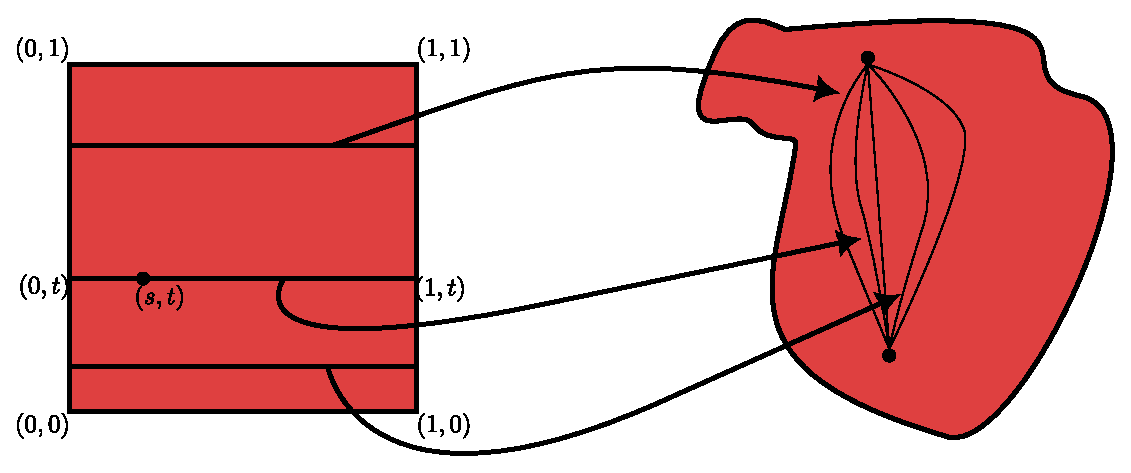
\includegraphics[scale=0.5]{Figures/path_prod.eps}
    \caption{Una homotopia relativa entre caminos.}
    \label{fig_21}
\end{figure}

\begin{definition}
    Sea $\partial{I}$ el borde de $I=[0,1]$. Llamaos las clases de equivalencias
    de la homotopia relativa $\simeq_{\partial{I}}$ \textbf{clases de caminos}.
    S\'i $f$ es un camino, denotamos el clase de caminos de  $f$ por  $[f]$.
\end{definition}

\begin{theorem}\label{11.32}
    Suponga que $f_0,f_1$ y $g_0,g_1$ son caminos en un espacio topologico $X$
    tales que  $f_0 \simeq f_1 \rel{\partial{I}}$ y $g_0 \simeq g_1
    \rel{\partial{I}}$. S\'i $f_0(1)=g_0(0)$ y $f_1(1)=g_1(0)$, entonces
    $f_0 \ast g_0 \simeq f_1 \ast g_1 \rel{\partial{I}}$.
\end{theorem}
\begin{proof}
    Sean $F:f_0 \simeq f_1 \rel{\partial{I}}$ y $G:g_0 \simeq g_1
    \rel{\partial{I}}$ homotopias relativas entres  $f_0$ y $f_1$, y $g_0$ y
    $g_1$. Defina la mapa $H:[0,1] \times [0,1] \xrightarrow{} Y$ dado por
    \begin{equation*}
     H(s,t)=\begin{cases}
                 F(2s,t), & \text{ s\'i } 0 \leq s \leq \frac{1}{2} \\
                 G(2s-1,t), & \text{ s\'i } \frac{1}{2} \leq s \leq 1   \\
            \end{cases}
    \end{equation*}
    Por el teorema del empaste, vemos que $H$ es continua, ademas vemos que
    $H(0,t)=F(0,t)=f_0 \ast g_0(t)$, y $H(1,t)=G(1,t)=f_1 \ast g_1(t)$. As\'i
    que $H:f_0 \ast g_0 \simeq f_1 \ast g_1 \rel{\partial{I}}$ es una homotopia
    relativa.
\end{proof}
\begin{corollary}
    $[f_0 \ast g_0]=[f_1 \ast g_1]$.
\end{corollary}

\begin{definition}
    S\'i $f:[0,1] \xrightarrow{} X$ es un camino con $x_0=f(0)$ y $x_1=f(1)$,
    entonces llamaos a $x_0$ el \textbf{origen} y $x_1$ el \textbf{final} de
    $f$, y lo denotamos por  $x_0=\alpha(f)$ y $x_1=\omega(f)$. Denotamos el
    origen y final del clase de caminos de ser $\alpha[f]=\alpha([f])$ y
    $\omega[f]=\omaga([f])$, respectivamente.
\end{definition}

\begin{definition}
    S\'i $f:[0,1] \xrightarrow{} X$ es un camino y $p$ es un punto en  $X$,
    entonces llamamos la mapa constante  $i_p:t \xrightarrow{} p$, para todo $t
    \in [0,1]$ el \textbf{camino constante}. Similarmente, llamamos al la mapa
    $\inv{f}(t)=f(1-t)$ el \textbf{camino inverso} de $f$.
\end{definition}

\begin{definition}
    Llamamos a un conjunto $G$, junto a una operacion binaria $\ast$ (no
    siempre definida) un \textbf{grupoide} s\'i
    \begin{enumerate}
        \item[(1)] $a \ast (b \ast c)=(a \ast b) \ast c$ s\'i $a \ast (b \ast
            c)$, o $(a \ast b) \ast c$ estan definidos, para todo $a,b,c \in G$.

        \item[(2)] Existen elementos $e_1,e_2 \in G$ tal que $a \ast e_1=a$ y
            $e_2 \ast a=a$; para todo $a \in G$.

            \item[(3)] Para toda $a \in G$, existe un elemento  $\inv{a} \in G$
                tal que $a \ast \inv{a}=e_1$ y $\inv{a} \ast a=e_2$.
    \end{enumerate}
\end{definition}

\begin{theorem}\label{11.34}
    S\'i $X$ es un espacio topologico, entonces el conjunto de todas las clases
    de caminos de  $X$ forman un grupoide bajo el producto de caminos. Es decir:
    \begin{enumerate}
        \item[(1)] El producto de caminos es associativa cuando esta definido
            apropiadamente.

        \item[(2)] S\'i $p=\alpha[f]$ y $q=\omega[f]$, entonces existen caminos
            constantes $i_p$ y $i_q$ tales que
            \begin{align*}
                [i_p][f]=f  &&  \text{y}   &&   [f][i_q]=[f]       \\
            \end{align*}

        \item[(3)] Para todo clase de camio $[f]$, existe el clase de camino
        $[\inv{f}]$ es tal que:
            \begin{align*}
                [f][\inv{f}]=[i_p]  &&  \text{y}    &&  [\inv{f}][f]=[i_q]  \\
            \end{align*}
            donde $p=\alpha[f]$ y $q=\omega[f]$.
    \end{enumerate}
\end{theorem}
\begin{proof}
    Dado $a,b \in \R$, defina la mapa $\theta_{[a,b]}:[a,b] \xrightarrow{}
    [0,1]$ dado por la regla
    \begin{equation*}
        \theta_{[a,b]}(s)=\frac{s-a}{b-a} \text{ para todo } s \in [a,b]
    \end{equation*}
    $\theta_{[a,b]}$ es una aplicaci\'on af\'in para todo $a,b \in \R$. Nota que
     $\theta_{[a,b]}(a)=0$ y $\theta_{[a,b]}(b)=1$. Mas a\'un, para cualquier
     camino $f$,  $f \circ \theta_{[a,b]}$ es continua.

     Sea $f:I \xrightarrow{} X$, $g:I \xrightarrow{} X$, y $h:I \xrightarrow{}
     X$ caminos donde $f(1)=g(0)$, $g(1)=h(0)$ y $(f \ast g) \ast h$, o $f \ast
     (g \ast h)$ estan definidos y considere la figura \ref{fig_22}.
     \begin{figure}[h]
         \centering
         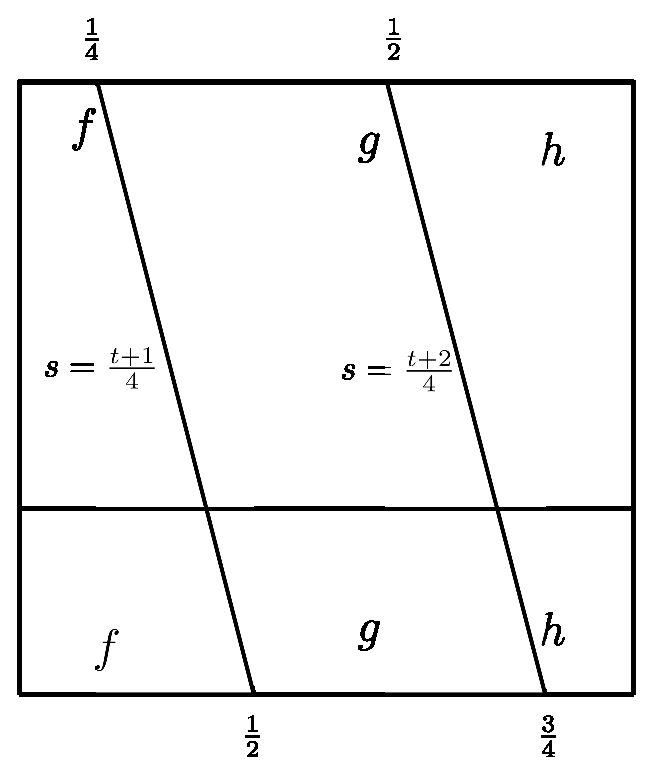
\includegraphics[scale=0.5]{Figures/path_associativity.eps}
         \caption{}
         \label{fig_22}
     \end{figure}
     Defina $H:I \times I \xrightarrow{} X$ dado por
     \begin{equation*}
          H(s,t)=\begin{cases}
                    f(\frac{4s}{1+t}), & \text{ s\'i } s \in [0,\frac{t+1}{4}] \\
                    g(4s-1-t), & \text{ s\'i } s \in [\frac{t+1}{4},\frac{t+2}{4}]   \\
                    h(1-\frac{4(1-s)}{2-t}), & \text{ s\'i } s \in [\frac{t+2}{4},1] \\
                 \end{cases}
     \end{equation*}
     $H$ es continua por el teorema del empaste. Mas a\'un $H(s,0)=(f \ast g)
     \ast h(s)$ y $H(s,1)=f \ast (g \ast h)(s)$. Por ultimo $H(0,t)=f(0)=p$ y
     $H(1,t)=h(1)=q$. Por lo tanto $(f \ast g) \ast h \simeq f \ast (g \ast h)
     \rel{partial{I}}$.

     Ahora, sea $[f]$ una clase de camino de $X$ con  $p=\alpha[f]$ y
     $q=\omega[f]$. Sean $i_p:t \xrightarrow{} p$ y $i_q:t \xrightarrow{} q$ los
     caminos constantes correspondiente a $p$ y $q$. Considere el sigueinte
     figura \ref{fig_23}

     \begin{figure}[h]
         \centering
         \includegraphics[scale=0.5]{Figures/path_identity.eps}
         \caption{}
         \label{fig_23}
     \end{figure}

     Defina la mapa $H:I \times I \xrightarrow{} X$ dado por
     \begin{equation*}
          H(s,t)=\begin{cases}
                    p, & \text{ s\'i } s \in [0,\frac{t}{2}]    \\
                    f(\theta_{[\frac{t}{2},1]}(s)), & \text{ s\'i } s \in
                    [\frac{t}{2},1]
                 \end{cases}
     \end{equation*}
     Note que $H(\frac{t}{2},t)=f(0)=p$, as\'i por el teorema del empaste, $H$
     es continua. Mas a\'un nota que $H(s,0)=f(s)$ y $H(s,1)=i_p \ast f$. Vemos
     tambien que $H(0,t)=p$ y $H(1,t)=f(1)=q$. Por lo tanto $i_p \ast f \simeq f
     \rel{\partial{I}}$. De igual manera, podemos ver que $f \ast i_q \simeq f
     \rel{\partial{I}}$.

     Por ultimo, sea $f$ un camino en $X$ con $p=\alpha(f)$ y $q=\omega(f)$.
     Considere el camino inverso $\inv{f}$, y construye la figura \ref{fig_24}.
     \begin{figure}[h]
         \centering
         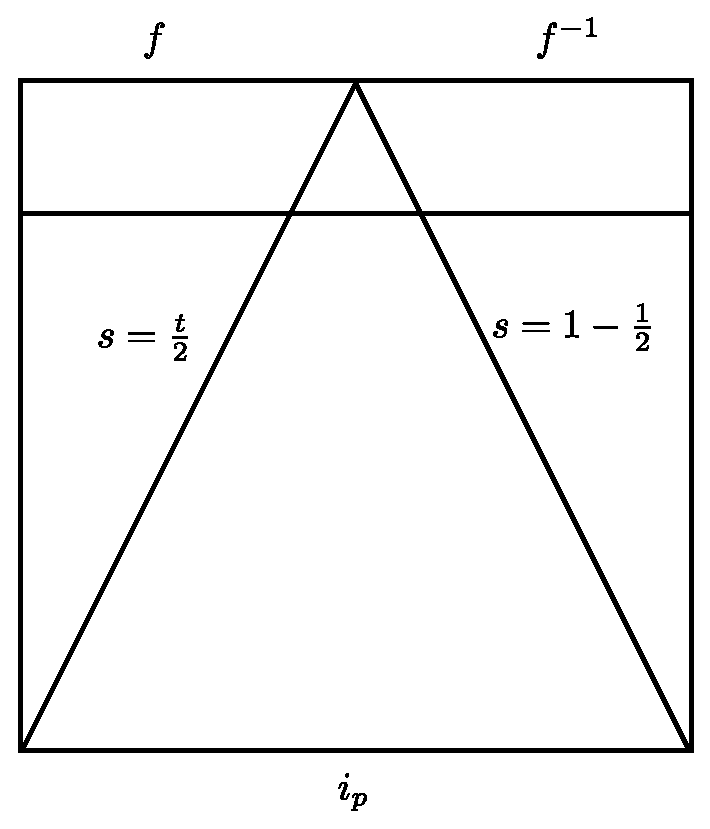
\includegraphics[scale=0.5]{Figures/path_inverse.eps}
         \caption{}
         \label{fig_24}
     \end{figure}
    Defina $H:I \times I \xrightarrow{} X$ por
    \begin{equation*}
          H(s,t)=\begin{cases}
                      f(2s), & \text{ s\'i } s \in [0, \frac{t}{2}]  \\
                      f(t), & \text{ s\'i } s \in [\frac{t}{2}, \frac{1-t}{2}] \\
                      \inv{f}(2(1-s)), &  \text{ s\'i } s \in [\frac{1-t}{2},1]  \\
                 \end{cases}
    \end{equation*}
    Nota que $H$ es continua por empaste. Mas a\'un, $H(s,0)=f(0)=p=i_p(s)$ y
    $H(s,1)=f \ast \inv{f}(s)$. Mas a\'un $H(0,t)=f(0)=p$ y
    $H(1,t)=\inv{f}(0)=q$. As\'i que $f \ast \inv{f} \simeq i_p
    \rel{\partial{I}}$. Similarmente, se halla que $\inv{f} \ast f \simeq i_q
    \rel{\partial{I}}$.
\end{proof}

\section*{Lectura 12: Anillos}

\begin{definition}
    Un \textbf{anillo} $R$ es un grupo abeliano bajo una operacion binaria  $+$
    junto a una operacion binarai $\cdot:(a,b) \xrightarrow{} ab$ tal que
    \begin{enumerate}
        \item[(1)] $\cdot$ es associativa.

        \item[(2)] $a(b+c)=ab+ac$ y $(a+b)c=ac+bc$.
    \end{enumerate}
    S\'i existe un elemento $1 \in R$ tal que  $a_1=1a=a$, entonces llamamos a
    $R$ un anillo con  \textbf{unidad}. Denotamos el elemento de identidad de
    $R$ bajo  $+$ como  $0$. S\'i $ab=ba$ para todo  $a,b \in R$, entonces
    llamamos  $R$  \textbf{commutativa}.
\end{definition}

\begin{definition}
    Sea $R$ un anillo con unidad, y  $a,b \in R$. S\'i $ab=0$ donde  $a\neq 0$,
     y $b \neq 0$, entonces llamamos a $a$ y  $b$  \textbf{divisores de cero}.
     S\' $ab=ba=1$, entonces llamamos a  $a$ y  $b$  \textbf{unidades}.
\end{definition}

\begin{definition}
    Un \textbf{dominio integral} es un anillo commutativa sin divisores de $0$.
    Llamamos la  \textbf{characteristica} de un anillo $R$ de ser el entero mas
    peque\~no $n$ tal que $na=\underbrace{a+\dots+a}_{n-\text{veces}}=0$, para
    todo $a \in R$.
\end{definition}

\begin{definition}
    Sean $R$ y  $S$ anillos. Llamamos a un mapa  $\phi:R \xrightarrow{} S$ un
    \textbf{homomorfismo de anillos} s\'i
    \begin{enumerate}
        \item[(1)] $\phi(a+b)=\phi(a)+\phi(b)$

        \item[(2)] $\phi(ab)=\phi(a)\phi(b)$
    \end{enumerate}
\end{definition}

\begin{example}\label{}
    \begin{enumerate}
        \item[(1)] Sea $\phi:\faktor{\Z}{6\Z} \xrightarrow{} \faktor{\Z}{6\Z}$
            dado por $n \xrightarrow{} 3n$. Entonces $\phi(x+y)=3(x+y)=3x+3y$ y
            $\phi(xy)=3(xy)=3x_3y$, como $3 \cdot 3 \equiv 3 \mod{6}$. As\'i que
            $\phi$ es un homomorfismo de anillos.
    \end{enumerate}
\end{example}

\section*{Lectura 13: Anillos Cocientes}

\begin{definition}
    Sea $R$ un anillo y $I$ un ideal, entonces $\faktor{R}{I}=\{r+I : r \in R\}$
    se llama el \textbf{anillo cociente} de $R$ sobre $I$.
\end{definition}

\begin{lemma}\label{13.56}
    Sea $R$ un anillo, y  $I$ un ideal, entonces el anillo cociente
    $\faktor{R}{I}$ es un anillo bajo la suma de $R$ y la multiplicacion $\cdot$
    dado por $(a+I,b+I) \xrightarrow{} (a+I)(b+I)=ab+I$.
\end{lemma}

\begin{lemma}\label{13.57}
    Todo ideal es el kernel de un homomorfismo de anillos.
\end{lemma}
\begin{proof}
    Escoje $\pi:R \xrightarrow{} \faktor{R}{I}$, entonces $\ker{\pi}=I$.
\end{proof}

\begin{theorem}[El Teorema del Factor]\label{13.58}
    Cualquier homomorfismo de anillis $\phi:R \xrightarrow{} S$ con kernel $K$
    que contiene a un ideal  $I$ se puede factorizarse via  $\faktor{R}{I}$,
    como $\phi=\bar{\phi} \circ \pi$ donde $\pi:R \xrightarrow{} \faktor{R}{I}$
    y $\bar{\phi}:\faktor{R}{I} \xrightarrow{} S$ es el unico homomorfismo con
    $\bar{\phi}$ sobre si y solo si $\phi$ es sobre y  $\bar{\phi}$ 1--1 si y
    solo si $K=I$.

    \[\begin{tikzcd}
	R &&& S \\
	\\
	\\
	{\faktor{R}{I}}
	\arrow["\phi", from=1-1, to=1-4]
	\arrow["{\bar{\phi}}"', from=4-1, to=1-4]
	\arrow["\pi"', from=1-1, to=4-1]
\end{tikzcd}\]

\end{theorem}

\begin{theorem}[Primer Teorema de Isomorfismo]\label{13.59}
    S\'i $\phi:R \xrightarrow{} S$ es un homomorfismo, entonces $\phi(R) \simeq
    \faktor{R}{K}$ donde $K=\ker{\phi}$.
\end{theorem}

\begin{theorem}[Segundo Teorema de Isomorfismo]\label{13.60}
    $\faktor{R+I}{I} \simeq \faktor{R}{R \cap I}$.
\end{theorem}

\begin{example}\label{}
    Considere $\phi:\R[x] \xrightarrow{} \C$ dado por $\phi(p(x))=p(i)$, la
    valuacion de $p$ en $i$. Entonces $\ker{\phi}=\{p(x) : p(i)=0\}=\R[x](x^2+1)$,
    como $i^2+1=0$, tenemos que $\faktor{\R[x]}{(x^2+1)} \simeq \C$.
\end{example}

\end{document}
